\newpage

\hypertarget{ux6253ux68cdux51faux7bb1}{%

%\subsection{\texorpdfstring{打棍出箱\footnote{ 刘曾复先生在协助王世续先生录制《打棍出箱》说戏录像时,配了其余角色,``出箱''一场的公差乙由李舒先生担任。。{492}}}{打棍出箱492}}\label{ux6253ux68cdux51faux7bb1}
}

{{[}第一场{]}}

{樵夫}\hspace{30pt}~

({\akai 念})人在桥上走,水在桥下流。老汉无别事,砍樵度春秋。

樵夫\hspace{30pt}~

老汉穆禾,{$\cdots{}\cdots{}$}砍樵。

樵夫\hspace{30pt}~

喂------伙计们,看今日天气晴和,我们何不往南山砍樵。

{(众\hspace{40pt}~

我们不去。)}

{樵夫\hspace{30pt}~

为何不去?}

{(众\hspace{40pt}~

南山有虎。)}

{樵夫\hspace{30pt}~

我腰掖板斧,怕它何来?}

{(众\hspace{40pt}~

要去你去,我们不去,让老虎啃你的老骨头。)}

{樵夫\hspace{30pt}~

呀呸!啃你们的老骨头。({\akai 或}: 怎么讲话呀!吃你们的老骨头。)}

{樵夫\hspace{30pt}~

你们不去({\akai 或}: 他们不去),待我一人前往。}

{樵夫

出得门来,好天气也------({\akai 或}: 出得门来,人倒老了呵,这景哟------)}

{樵夫

\setlength{\hangindent}{60pt}{ 【}四平调{】八十岁老翁进花园,手攀花枝泪涟涟。花开花落无长久,人过青呐 }

春无有少年。}

{樵夫\hspace{30pt}~

来此已是南山,待我用起功来。}

{范仲禹} ({\akai 内}){走哇!}

范仲禹\hspace{20pt}~

\setlength{\hangindent}{60pt}{ 【{\akai 二黄散板}】山前山后我俱找到,不见妻儿啊为哪条? }

范仲禹

卑人,府学生员范仲禹。今当大比之年,(带领妻室、孩儿)\footnote{ 此处及以下括号中范仲禹的念白根据吴焕老师整理的剧本(经刘曾复先生审订)添加。{493}}进京会试。前半

月,在此处失落了妻室、孩儿。是我山前、山后,寻找半月,并无踪影。只是

教我哪里去寻,哪里------唉!去找$\cdots{}\cdots{}$哇,呃$\cdots{}\cdots{}$(哭介)

{樵夫\hspace{30pt}~

------砍樵哦$\cdots{}\cdots{}$}

{范仲禹} 看那旁有一樵夫,待我上前问呐来。

范仲禹\hspace{20pt}~

嘿,樵哥,这里来,我有话对你讲啊。

范仲禹\hspace{20pt}~

不曾听见,待我那厢去唤。

范仲禹\hspace{20pt}~

嘿,樵哥,这里来,我有话对你讲啊。

范仲禹\hspace{20pt}~

诶,是一个聋子啊。

范仲禹\hspace{20pt}~

待我来吓他一吓。

范仲禹\hspace{20pt}~

嗷呜------

{樵夫\hspace{30pt}~

看斧------}

{樵夫

呀呸!$\cdots{}\cdots{}$我这一斧将你劈死,是斧你的偿命呢,还是人偿你的命呢?}

{范仲禹\hspace{20pt}~

哎呀,樵哥哇!}

{樵夫\hspace{30pt}~

站远些。}

范仲禹\hspace{20pt}~

你在此处砍樵,可曾看见我的儿子啊?

{樵夫

呀呸!$\cdots{}\cdots{}$我在这看樵好好,哪个晓得你那儿子是个高子啊,是个矮子啊;是个胖子

啊,喏喏喏,是个瘦子呢?}

范仲禹\hspace{20pt}~

此乃是前半月的事啊。

樵夫\hspace{30pt}~

怎么,是前半月的事------这这这{$\cdots{}\cdots{}$}

{樵夫\hspace{30pt}~

呃,有的啊------}

范仲禹\hspace{20pt}~

有的?

樵夫\hspace{30pt}~

有的------

范仲禹\hspace{20pt}~

有的?!

樵夫、范仲禹 啊,呵哈哈哈$\cdots{}\cdots{}$(笑介)

樵夫、范仲禹 有的。

樵夫、范仲禹 有的。

樵夫、范仲禹 啊,呵呵哈哈哈$\cdots{}\cdots{}$(笑介)

范仲禹\hspace{20pt}~

有在哪里?

樵夫

相公听了: 前半月,在这大路旁边,有一小小的顽童,是这样哭哭啼啼。南山

上,下来一只猛虎,将那顽童,嗷呜就衔呐------衔在口内。

范仲禹

樵哥: 前半月,在这大路旁边,有一小小的顽童,是这样哭哭啼啼。南山上,

下来一只猛虎,将那顽童,嗷呜就衔呐------衔在口内。

范仲禹\hspace{20pt}~

樵哥,

樵夫\hspace{30pt}~

怎么。

范仲禹\hspace{20pt}~

儿啊$\cdots{}\cdots{}$(哭介)

樵夫\hspace{30pt}~

诶------你是怎么讲话?你那儿子啊,他还有救啊。

范仲禹\hspace{20pt}~

还有救啊?

樵夫\hspace{30pt}~

有救。

范仲禹\hspace{20pt}~

有救?

樵夫\hspace{30pt}~

有救。

范仲禹\hspace{20pt}~

有救?!

樵夫、范仲禹 啊,呵哈哈哈$\cdots{}\cdots{}$(笑介)

范仲禹\hspace{20pt}~

有救?

樵夫\hspace{30pt}~

有救。

范仲禹\hspace{20pt}~

有救?!

樵夫\hspace{30pt}~

有救。

樵夫、范仲禹 啊,呵哈哈哈$\cdots{}\cdots{}$(笑介)

范仲禹\hspace{20pt}~

救在哪里?

樵夫

相公听了: 我们这里,有一打虎的壮士,名唤陆荣,见那猛虎口衔顽童,赶上

前去,是这样三拳两足,将虎打走,就是这样背呀------背回家去。

范仲禹

樵哥: 你们这里,有一打虎的壮士,名唤陆荣,见那猛虎口衔顽童,赶上前去,

是这样三拳两足,将虎打走,就是这样背呀------背回家去。

范仲禹\hspace{20pt}~

呵呵哈哈哈$\cdots{}\cdots{}$(笑介)

范仲禹\hspace{20pt}~

且喜儿子有了下落了,待我来谢天谢地!

樵夫\hspace{30pt}~

当谢天地。

范仲禹\hspace{20pt}~

啊,樵哥,辛苦你了!

樵夫\hspace{30pt}~

嗯,好说。

范仲禹\hspace{20pt}~

难为你了!

樵夫\hspace{30pt}~

这是哪里的话呀。

范仲禹\hspace{20pt}~

我啊,我要走了哇。

樵夫\hspace{30pt}~

哦,那那你走吧。

范仲禹\hspace{20pt}~

我要走了哇!

樵夫\hspace{30pt}~

你走吧。

范仲禹\hspace{20pt}~

诶呀------儿子有了下落,还有他儿子的娘呐!

范仲禹\hspace{20pt}~

待我来再问一问,儿子他的娘呃。

范仲禹\hspace{20pt}~

嘿,樵哥,这里来,我还有话对你讲啊。

范仲禹\hspace{20pt}~

还是不曾听见,我再来吓他一吓。

范仲禹\hspace{20pt}~

嗷呜------

{樵夫\hspace{30pt}~

打虎------}

{樵夫\hspace{30pt}~

看斧------嘿,你怎么又回来了!}

范仲禹\hspace{20pt}~

哎呀,樵哥哇!

{樵夫\hspace{30pt}~

诶,你站远些。}

范仲禹\hspace{20pt}~

你既然晓得儿子的下落,你可晓得儿子他的娘啊?

{樵夫

呀呸!$\cdots{}\cdots{}$晓得儿子的下落,哪里有什么儿子他的娘啊。}

范仲禹\hspace{20pt}~

也是前半月的事啊。

樵夫\hspace{30pt}~

哦哦哦,也是前半月的事------

樵夫\hspace{30pt}~

呃呃呃,有的啊------

范仲禹\hspace{20pt}~

有的?

樵夫\hspace{30pt}~

有的。

范仲禹\hspace{20pt}~

有的?!

樵夫\hspace{30pt}~

有的。

樵夫、范仲禹 啊,呵哈哈哈$\cdots{}\cdots{}$(笑介)

范仲禹\hspace{20pt}~

有的。

樵夫\hspace{30pt}~

有的。

范仲禹\hspace{20pt}~

有的。

樵夫\hspace{30pt}~

有的。

樵夫、范仲禹 啊,呵呵哈哈哈$\cdots{}\cdots{}$(笑介)

范仲禹\hspace{20pt}~

有在哪里?

樵夫

相公听了: 前半月,在这大路旁边,有一女娘行,也是这样啼啼哭哭。我们这

里有一告老的太师,带领家下人等,是游山观景。观见那女娘行,吩咐掌起面

来\footnote{\hspace{10pt}~

段公平君建议作``张起面来''。{494}},就

觑呀------有几分姿首\footnote{ 姿首,指美丽的容貌,也可泛指容貌。{495}},吩咐家下人等,就背呃------背回家去。

范仲禹

樵哥: 前半月,在这大路旁边,有一女娘行,也是这样啼啼哭哭。你们这里有

一告老的太师,带领家下人等,是游山观景。观见那女娘行,吩咐掌起面来,

就觑呀------有几分姿首,吩咐家下人等,就背呃------背回家去。

范仲禹\hspace{20pt}~

呵呵哈哈哈$\cdots{}\cdots{}$(笑介)

范仲禹\hspace{20pt}~

且喜儿子他的娘也有了下落了,待我来再谢天谢地!

樵夫

呵呵,你看他还要谢天地,想那告老太师乃是个酒色之徒。白日饮酒,到了晚

上么$\cdots{}\cdots{}$呃,呃,呃$\cdots{}\cdots{}$

范仲禹\hspace{20pt}~

坏了!

樵夫\hspace{30pt}~

不曾------

范仲禹\hspace{20pt}~

坏了,坏了哇!

樵夫\hspace{30pt}~

不曾呐。

范仲禹\hspace{20pt}~

坏了!

樵夫\hspace{30pt}~

不曾------

范仲禹\hspace{20pt}~

坏了,唉,坏了哇!

樵夫\hspace{30pt}~

不曾呐。

范仲禹\hspace{20pt}~

这个老贼,他叫什么名字?

樵夫\hspace{30pt}~

他叫葛$\cdots{}\cdots{}$呃,呃,呃。

范仲禹\hspace{20pt}~

你为何不讲?

樵夫\hspace{30pt}~

我不敢言讲。

范仲禹\hspace{20pt}~

你为何不敢言讲?

樵夫

前番有人叫他的名字,送到有司衙门,责打四十大板,齐眉毛的,倒还要充军。

范仲禹\hspace{20pt}~

哪有这大的罪过?

樵夫\hspace{30pt}~

这叫作``死不饶人''呐。

范仲禹\hspace{20pt}~

樵哥,你看这山前、山后,就是你我二人,但讲何妨?

樵夫\hspace{30pt}~

哦,怎么------讲得的。

范仲禹\hspace{20pt}~

樵哥,讲得的。

樵夫\hspace{30pt}~

你近前来。

范仲禹\hspace{20pt}~

你高声些。

樵夫\hspace{30pt}~

他叫$\cdots{}\cdots{}$(低声)

范仲禹\hspace{20pt}~

高声些。

樵夫\hspace{30pt}~

你是个聋子呀。

范仲禹\hspace{20pt}~

你是个哑子啊!

范仲禹\hspace{20pt}~

他叫什么名字?

范仲禹\hspace{20pt}~

高声些。

樵夫\hspace{30pt}~

他叫$\cdots{}\cdots{}$(低声)

范仲禹\hspace{20pt}~

高声些。

樵夫\hspace{30pt}~

诶,你是个聋子呀。

范仲禹\hspace{20pt}~

哎呀,你是个哑子啊!

樵夫\hspace{30pt}~

他叫$\cdots{}\cdots{}$(低声)

范仲禹\hspace{20pt}~

他到底叫什么?

樵夫\hspace{30pt}~

诶------他,他$\cdots{}\cdots{}$他叫葛登云?!

范仲禹\hspace{20pt}~

哦------他,他$\cdots{}\cdots{}$他叫葛登云?!

范仲禹\hspace{20pt}~

他住在哪里?

樵夫\hspace{30pt}~

哎------呀!一不做二不休,打贼不死反成仇。来来来,随我来呀------

樵夫\hspace{30pt}~

就在前面,八字粉墙,合脊门楼,金字牌匾,两柱大旗杆,就是贼府?!

范仲禹\hspace{20pt}~

就在前面,八字粉墙,合脊门楼,金字牌匾,两柱大旗杆,就是贼府?!

范仲禹\hspace{20pt}~

告辞了!

樵夫\hspace{30pt}~

喂呀呀$\cdots{}\cdots{}$相公此去,定有一番热闹。

樵夫

哎呀不好!倘若那太师爷问起,是何人对你讲的,他若说出我来------哎呀,这还

了得$\cdots{}\cdots{}$哎呀,这这这$\cdots{}\cdots{}$

樵夫\hspace{30pt}~

唉,待我唤他回来。嘱咐几句。

樵夫\hspace{30pt}~

诶------

范仲禹\hspace{20pt}~

哙!去远了啊!

樵夫\hspace{30pt}~

你回来呀------

范仲禹\hspace{20pt}~

我走得好好,你唤我回来则甚呐?

樵夫\hspace{30pt}~

呃,此番见了太师,太师若问,何人同你讲的,你是怎样回答?

范仲禹\hspace{20pt}~

呵呵哈哈哈$\cdots{}\cdots{}$(笑介)

范仲禹\hspace{20pt}~

那我还难为得了你么?

樵夫\hspace{30pt}~

你怎样讲?

范仲禹\hspace{20pt}~

我啊,我就说: 你对我讲的。

樵夫\hspace{30pt}~

诶------你把话还我罢。

范仲禹\hspace{20pt}~

呀呸!话出如风,怎能还你?

樵夫\hspace{30pt}~

倘若太师问起,你就说你是亲眼得见。

范仲禹

樵哥!老贼不问起便罢;倘若问起,我就说我亲呐------眼,亲呐------眼------得见。

范仲禹\hspace{20pt}~

樵哥!

樵夫\hspace{30pt}~

诶,做什么?

范仲禹\hspace{20pt}~

儿啊$\cdots{}\cdots{}$(哭介)

樵夫\hspace{30pt}~

诶,这是怎么讲话呀。

樵夫\hspace{30pt}~

哎呀,我看此处不是我久留之处。待我收拾收拾,逃往他乡去吧。(kai 正是}: 

樵夫\hspace{30pt}~

({\akai 念})双手劈开生死路,翻身呐------逃出是非墙。

{{[}第二场{]}}

范仲禹\hspace{20pt}~

\textless{}\!{\bfseries\akai 哭头}\!\textgreater{}啊,我的儿啊!

范仲禹\hspace{20pt}~

我有事啊,诶------我有事啊!

范仲禹

\setlength{\hangindent}{60pt}{ 【{\akai 二黄散板}】恨贼子把我的牙咬断,霸抢民妻礼不端。迈开大步朝前趱呐, }

范仲禹\hspace{20pt}~

\setlength{\hangindent}{60pt}{ 【{\akai 二黄散板}】不觉来到贼的府门前。 }

范仲禹

八字粉墙,合脊门楼({\akai 或}: 乌脊门楼),金字的牌匾呐,喏喏喏,还有两柱大旗

杆。

范仲禹\hspace{20pt}~

嗯,是这里。

范仲禹\hspace{20pt}~

呔,有人么?走出一个来呀!

家院\hspace{30pt}~

门外啰唣,有人来到。

家院\hspace{30pt}~

什么人?

范仲禹\hspace{20pt}~

你可姓葛?

家院\hspace{30pt}~

我姓葛。

范仲禹\hspace{20pt}~

着打!

家院\hspace{30pt}~

你怎么打起我来了?

范仲禹\hspace{20pt}~

你可是葛登云?

家院\hspace{30pt}~

呃,那是我家相爷。

范仲禹\hspace{20pt}~

哎呀,打错了。老贼可在府内?

家院\hspace{30pt}~

呃,现在书房。

范仲禹\hspace{20pt}~

与你大相公牵了出来!

家院\hspace{30pt}~

呃------请了出来。

范仲禹\hspace{20pt}~

牵了出来!

家院\hspace{30pt}~

请了出来。

家院\hspace{30pt}~

下站!

家院\hspace{30pt}~

有请相爷。

葛登云\hspace{20pt}~

呃------哼!

(痰嗽)

葛登云\hspace{20pt}~

({\akai 念})身为当朝首相,喜爱美貌娇娘。

葛登云\hspace{20pt}~

何事?

家院\hspace{30pt}~

有一疯汉,打上府门。

葛登云\hspace{20pt}~

家丁们走上。

葛登云\hspace{20pt}~

待我看来------

葛登云\hspace{20pt}~

疯汉在哪里,疯汉在------

范仲禹\hspace{20pt}~

啊,老太师你好哇?

葛登云\hspace{20pt}~

呃我好,你可好?

范仲禹\hspace{20pt}~

我么,唉,还好,还好哇!

范仲禹\hspace{20pt}~

啊,老太师你好福气呀!

葛登云\hspace{20pt}~

呃,夸奖了。

范仲禹\hspace{20pt}~

你好贵相啊!

葛登云\hspace{20pt}~

呃------

范仲禹\hspace{20pt}~

老太师,喏喏喏,你好长的胡须呀!

葛登云\hspace{20pt}~

呜哟------

葛登云\hspace{20pt}~

你是何人?

范仲禹\hspace{20pt}~

呀呸!府学生员范仲禹,范大相公就是我哇!

葛登云\hspace{20pt}~

大胆疯汉,打到老夫我的府门是何缘故?

范仲禹

我把你这个老狗!别人家的妻室,你可以霸占得,范仲禹,范大相公的妻子,也是你这个老狗霸占得不成?快快还我妻子便罢,不然呐,我就打死你这个老狗!

葛登云\hspace{20pt}~

此话何人对你讲的?

范仲禹\hspace{20pt}~

此乃山中樵$\cdots{}\cdots{}$

葛登云\hspace{20pt}~

呃,将山中樵夫送至有司衙门。

范仲禹\hspace{20pt}~

哎呀樵哥,事到如今,我也顾不得你了。

范仲禹\hspace{20pt}~

此乃山中樵夫,对我言讲。还有什么假的不成?

葛登云

啊,范相公哪里知道,那山中樵夫,偷盗老夫的树木,将他送在有司衙门。

范仲禹\hspace{20pt}~

放屁!

葛登云\hspace{20pt}~

他在范大相公面前,搬动是非。

范仲禹\hspace{20pt}~

好臭好臭!

葛登云\hspace{20pt}~

啊,范相公,老夫乃是当朝首相,哪里无有三房四妻,焉能霸占你的妻子?

范仲禹\hspace{20pt}~

真真臭而不可闻也呀!

葛登云\hspace{20pt}~

有道是``傍耳之言,不可深信''。你要再思啊再想------

范仲禹\hspace{20pt}~

是啊!想他乃是告老太师,三四房妻妾总是有的呀,焉能霸占别人的妻子?

范仲禹\hspace{20pt}~

哎呀樵哥,这是我上了你的当了啊。

范仲禹\hspace{20pt}~

哎呀,打上人家的府门,这这这$\cdots{}\cdots{}$

范仲禹\hspace{20pt}~

唉,赔个礼儿可也就拉倒了。

范仲禹\hspace{20pt}~

啊------

葛登云\hspace{20pt}~

呃,呃$\cdots{}\cdots{}$

范仲禹\hspace{20pt}~

老太师!

范仲禹\hspace{20pt}~

呃,不打了!

葛登云\hspace{20pt}~

不打了。

范仲禹\hspace{20pt}~

得罪了老太师,我这厢赔礼了!

葛登云\hspace{20pt}~

不知者不见罪。

范仲禹\hspace{20pt}~

告辞!

葛登云\hspace{20pt}~

哪里去?

范仲禹

去至山前、山后,寻找我那妻室,唉,孩儿啊,呃$\cdots{}\cdots{}$(哭介)

葛登云\hspace{20pt}~

啊范相公,你看今日天色已晚,就在府中暂住一宵,明日差人寻访就是。

范仲禹\hspace{20pt}~

萍水相逢,怎好打搅?

葛登云\hspace{20pt}~

四海之内皆为朋友。

范仲禹\hspace{20pt}~

如此打搅不当了!

众\hspace{40pt}~

关大门。

葛登云\hspace{20pt}~

请------

众\hspace{40pt}~

关二门。

葛登云\hspace{20pt}~

请------

葛登云\hspace{20pt}~

请坐。

葛登云

\setlength{\hangindent}{60pt}{ 【{\akai 二黄原板}】太师府摆酒宴开怀畅饮,尊一声范相公细听分明: 今夜晚在府中安歇停顿({\akai 或}: 今夜晚在府中暂且安顿),到明天差人役前去找寻。\footnote{ 刘曾复先生在说《李陵碑》时顺便说了这几句。{496}} }

范仲禹\hspace{20pt}~

唉!

范仲禹\hspace{20pt}~

\setlength{\hangindent}{60pt}{ 【{\akai 二黄原板}】我本是一穷儒太烈性,冒犯了老太师府门呐庭。 }

范仲禹

\setlength{\hangindent}{60pt}{ 【{\akai 二黄原板}】怜卑人结发糟糠多薄命\footnote{ 李楠君所学作``结发糟糠多薄幸''。{497}},浪打鸳鸯两离分。 }

葛登云\hspace{20pt}~

请------

葛登云\hspace{20pt}~

大杯伺候。

范仲禹\hspace{20pt}~

\setlength{\hangindent}{60pt}{ 【{\akai 二黄原板}】我往日饮酒酒不醉,到今日饮酒酒醉人。 }

葛登云\hspace{20pt}~

搀至书房。

葛登云\hspace{20pt}~

葛虎进见。

葛虎\hspace{30pt}~

({\akai 念})堂上一呼,堂下百喏。

葛虎\hspace{30pt}~

相爷有何差遣?

葛登云\hspace{20pt}~

老夫平日待你如何?

葛虎\hspace{30pt}~

相爷待小人恩重如山。

葛登云\hspace{20pt}~

今有钢刀一把,去至书房将范仲禹杀来见我。

葛虎\hspace{30pt}~

遵命。

葛登云\hspace{20pt}~

转来,有何为证?

葛虎\hspace{30pt}~

钢刀见血为证。

葛登云\hspace{20pt}~

({\akai 念})此去莫追悔,

葛虎\hspace{30pt}~

({\akai 念})钢刀见血回。

{{[}第三场{]}}

(煞神起霸)

煞神

({\akai 念})嘴似钢锥牙似钉,二目睁睁似鸾铃。奉了上天玉帝旨,葛府搭救文曲星。

煞神\hspace{30pt}~

吾乃煞神是也,奉了玉帝敕旨,前去搭救,就此前往。

{{[}第四场{]}}

范仲禹\hspace{20pt}~

啊,老太师,卑人这酒么,是吃不得了。

范仲禹\hspace{20pt}~

吃不得了哇。

范仲禹\hspace{20pt}~

(呜哙呀,)好一座洁净的书房。

范仲禹

唉,悔不该听信樵夫之言,打上人家的府门。好个仁义的太师,非但不降罪于我,反是这样款待,思想起来,真是难得呀,难呐得!

范仲禹

\setlength{\hangindent}{60pt}{ 【四平调】听谯楼打罢了初更时分,忽然想起小娇生。我叫一声呐范金儿,你来了吧------我的儿啊!送儿到学中攻读书文呐,啊,攻读书文呐。 }

(煞神拍桌子叫醒范仲禹)

范仲禹\hspace{20pt}~

呃------哼!(痰嗽)

范仲禹\hspace{20pt}~

这书房之中,为何阴风惨惨?莫非有鬼么?!

范仲禹

\setlength{\hangindent}{60pt}{ 【四平调】耳边厢又听得二更尽,忽然想起结发情呐。我叫一声陆氏妻,你哪里去,我的妻呀!夫妻们见面叙一叙苦情呐,啊,叙一叙苦情呐。 }

(煞神拍桌子叫醒范仲禹,范仲禹见煞神)

范仲禹\hspace{20pt}~

呃------哼!

(痰嗽)

范仲禹

这书房之中,为何这样阴风惨惨,鬼哭神嚎?范仲禹呀范仲禹,只怕你性命,难逃今晚!

范仲禹\hspace{20pt}~

呃------哼!

(痰嗽)

范仲禹

\setlength{\hangindent}{60pt}{ 【四平调】三更三点白露茫,怎不教人泪两行。似风筝断了那无情线,我那妻儿啊!好一似无情浪打鸳鸯,啊,浪打鸳鸯。 }

葛虎\hspace{30pt}~

({\akai 念})阎王叫你三更死,岂能留你到五更!

葛虎\hspace{30pt}~

看刀!

(煞神杀葛虎,煞神拍桌子叫醒范仲禹)

家院\hspace{30pt}~

啊老太师,葛虎被人杀死!有请太师。

(众\hspace{40pt}~

有请太师。)

葛登云\hspace{20pt}~

何事?

家院\hspace{30pt}~

葛虎被人杀死。

葛登云\hspace{20pt}~

家丁们走上。待我看来。

葛登云\hspace{20pt}~

将他唤醒。

范仲禹\hspace{20pt}~

吓煞我也!吓煞我也!

葛登云\hspace{20pt}~

唗,胆大疯汉,为何将我家人杀死。

范仲禹\hspace{20pt}~

好贼({\akai 或}: 呀呸)!

范仲禹

({\akai 念})\textless{}\!{\bfseries\akai 扑灯蛾}\!\textgreater{}贼子理不端,理不端!强把民妻占!此处与你难分辩,有司衙门走一番!

葛登云\hspace{20pt}~

来,搭至南楼。

家院\hspace{30pt}~

他妻子现在南楼,若是相见,有些不便。

葛登云\hspace{20pt}~

依你之见。

家院\hspace{30pt}~

$\cdots{}\cdots{}$搭至荒郊,用火焚化$\cdots{}\cdots{}$

葛登云\hspace{20pt}~

安排下去。

葛登云\hspace{20pt}~

范仲禹啊范仲禹,

葛登云\hspace{20pt}~

({\akai 念})天堂有路你不走,地狱无门闯进来。

{{[}第五场{]}}

公差甲、公差乙 啊------哎------

公差甲\hspace{20pt}~

({\akai 念})中状元扬名天下

公差乙\hspace{20pt}~

({\akai 念})琼林宴何处寻他。

公差甲

哎,我说伙计哎,咱们都出来这么些个日子,这盘费都花光了,你看这怎么办呢这个事儿?

公差乙\hspace{20pt}~

我倒有个主意。

公差甲\hspace{20pt}~

你有什么高招儿?

公差乙\hspace{20pt}~

您瞧见这个没有,咱们就吃它了。

公差甲\hspace{20pt}~

我也没有好牙口啊。

公差乙你

呃不是啊,这有过往的客商啊,咱们搂头就一棍子,有钱有银子的,归了咱们,咱们不就有钱花了吗?

公差甲\hspace{20pt}~

咱们干什么的?

公差乙\hspace{20pt}~

咱们是当差的呀。

公差甲\hspace{20pt}~

当差的这叫干嘛啊------

公差乙\hspace{20pt}~

呃$\cdots{}\cdots{}$

公差甲\hspace{20pt}~

这叫``知法犯法,罪加一等''。

公差乙\hspace{20pt}~

呃,咱们就这一回,下不为例。

公差甲\hspace{20pt}~

咱们可就这一回了。

公差乙\hspace{20pt}~

诶,就这一回。

(众\hspace{40pt}~

走,走,走,走!)

公差甲\hspace{20pt}~

嘿你瞧,咱们这还有开张了。

公差乙\hspace{20pt}~

来了来了。

(四家丁抬箱上。公差甲、公差乙打,四家丁下)

公差甲\hspace{20pt}~

您瞧这什么了?当铺搬家?这是当铺搬家。

公差乙\hspace{20pt}~

哎,当铺搬家这是。

公差甲\hspace{20pt}~

诶------别忙别忙,咱们得念点喜歌。

公差乙\hspace{20pt}~

咱们打开看看。

公差甲\hspace{20pt}~

打开之后先摸,摸着什么是什么,不许换的。

公差乙\hspace{20pt}~

对。

公差甲\hspace{20pt}~

咱们呐,先念个喜歌吧。

公差乙\hspace{20pt}~

诶------

公差甲\hspace{20pt}~

开箱------

公差乙\hspace{20pt}~

大吉。

公差甲\hspace{20pt}~

万事------

公差乙\hspace{20pt}~

亨通。

公差甲\hspace{20pt}~

羊油------

公差乙\hspace{20pt}~

穿蜡。

公差甲\hspace{20pt}~

得了得了。

公差甲、公差乙 哎------摸起来------

公差甲\hspace{20pt}~

摸着没有啊?

公差乙\hspace{20pt}~

我摸着了。

公差甲

先瞧我的------嘿,你瞧诶,我这酒壶,我就好喝一杯。我瞧你的,这是什么?

公差乙\hspace{20pt}~

蜡扦。这是没用。

公差甲\hspace{20pt}~

换换。

公差乙\hspace{20pt}~

可以换换。

公差甲\hspace{20pt}~

摸着没有啊?

公差乙\hspace{20pt}~

我摸着了。

公差甲\hspace{20pt}~

还是先瞧我的------

公差乙\hspace{20pt}~

先瞧您的。

公差甲\hspace{20pt}~

嘿,我这可是有用的,你瞧诶,我这一串钱。我瞧你的,你这是什么票子?

公差乙\hspace{20pt}~

小鞋子。

公差甲\hspace{20pt}~

还得换换。

公差乙\hspace{20pt}~

还得换换。

公差甲\hspace{20pt}~

摸着没有啊?

公差乙\hspace{20pt}~

哎哟这可不得了,这怎么这么沉。

公差甲\hspace{20pt}~

先瞧你的------还是先瞧我的。你瞧这个,

公差乙\hspace{20pt}~

您发财了。

公差甲\hspace{20pt}~

这是手铐,我以为是眼镜呢。

公差乙\hspace{20pt}~

嗨。

公差甲\hspace{20pt}~

得了,这回咱别换了,还接着来。

公差乙\hspace{20pt}~

别换了。

公差甲\hspace{20pt}~

摸着没摸着啊?

公差乙\hspace{20pt}~

摸着了。

公差甲\hspace{20pt}~

这回啊,我一点不要了,都归您了------

公差乙\hspace{20pt}~

我也不要了。

范仲禹\hspace{20pt}~

\setlength{\hangindent}{60pt}{ 【四平调】在城隍庙中挂了号,土地祠内领回文,啊,领回文。 }

公差甲\hspace{20pt}~

诶哟我的妈呀------

公差乙\hspace{20pt}~

这什么毛病。

公差甲\hspace{20pt}~

这什么玩意儿?这都怎么了?

公差乙\hspace{20pt}~

这是什么玩意儿?

公差甲\hspace{20pt}~

诶,你别说,你不知道是吧。

公差乙\hspace{20pt}~

不知道。

公差甲\hspace{20pt}~

这我倒认得,这叫啊------``旱魃''。

公差乙\hspace{20pt}~

``旱魃''。

公差甲\hspace{20pt}~

诶------你别瞧这个,这个玩意啊,天一旱就出来。

公差乙\hspace{20pt}~

哦。

公差甲

诶,我还真喂过,这个玩意。你瞧着啊,它这个,它一逗啊,蹄、爪乱动,可有玩意了,可有意思了。待我来啊------

公差乙\hspace{20pt}~

哦。

公差甲\hspace{20pt}~

逗逗它。

公差乙\hspace{20pt}~

好。

公差甲\hspace{20pt}~

诶。他转身,拿这棍儿------

公差乙\hspace{20pt}~

有意思啊,有意思。

公差甲\hspace{20pt}~

唉呀我的妈呀------这里可没什么意思了,这个。

范仲禹\hspace{20pt}~

你骂了我了!

公差甲\hspace{20pt}~

谁骂你了。

公差乙\hspace{20pt}~

嗯,他骂你来着。

范仲禹\hspace{20pt}~

他骂了我了!

公差甲\hspace{20pt}~

谁骂你了。

公差乙\hspace{20pt}~

你骂他来着。

范仲禹\hspace{20pt}~

你骂了我了哇------

公差甲\hspace{20pt}~

你胡说,你怎么胡说啊。

公差乙\hspace{20pt}~

可不是。咱们俩可不是骂他来着?

范仲禹\hspace{20pt}~

\setlength{\hangindent}{60pt}{ 【四平调】你骂我是一个狂书生,平白骂我所为何情,啊,所为何情? }

公差甲\hspace{20pt}~

这没什么意思,不行,这可没啥意思了,不行,这个。

公差乙\hspace{20pt}~

它不是``旱魃''。

公差甲\hspace{20pt}~

那是什么啊?

公差乙\hspace{20pt}~

呃------它是``海怪''。

公差甲\hspace{20pt}~

什么``海怪''啊?

公差乙\hspace{20pt}~

这玩意儿,我喂过它。

公差甲\hspace{20pt}~

你喂过这个?

公差乙\hspace{20pt}~

诶------拿棍儿一逗啊,眉、尾乱动。

公差甲\hspace{20pt}~

哦?

公差乙\hspace{20pt}~

你瞧,你瞧我试试啊。

公差甲\hspace{20pt}~

我瞧你的!

公差乙\hspace{20pt}~

诶------

公差甲\hspace{20pt}~

它可真有个意思啊。

公差乙\hspace{20pt}~

有意思吧------

公差甲\hspace{20pt}~

有意思啊------您起来吧。

范仲禹\hspace{20pt}~

你打了我了!

公差乙\hspace{20pt}~

谁打你了?

范仲禹\hspace{20pt}~

他打了我了!

公差乙\hspace{20pt}~

啊,是他打你来着,你看看,脑袋上都流血了。

范仲禹\hspace{20pt}~

哎,你打我了哇------

公差甲\hspace{20pt}~

别胡说八道了!

范仲禹

\setlength{\hangindent}{60pt}{ 【四平调】我和你一无冤仇二无有怨恨,打我皮破鲜呐血淋,啊,鲜血淋。 }

公差甲

哎呀,我这个,我这明白了,这人啊。大概是让人给打了。这么着吧,咱们劝劝他吧。

公差甲、公差乙 劝劝他。

公差甲\hspace{20pt}~

\setlength{\hangindent}{60pt}{ 【四平调】是何人将你的头打破,你去寻找对头人,啊,对头人。 }

公差甲

你瞧是不是?诶,话是开心的钥匙,你瞧他就势------明白了。诶,你瞧,他走他的,咱们哥俩走咱们哥俩的。

公差甲\hspace{20pt}~

哦哟,哦哟,哦哟嚯。

范仲禹\hspace{20pt}~

你是我的儿子啊。

范仲禹\hspace{20pt}~

他是我的儿子啊。

范仲禹\hspace{20pt}~

唉,儿呀,啊$\cdots{}\cdots{}$(哭介)

范仲禹\hspace{20pt}~

\setlength{\hangindent}{60pt}{ 【四平调】叫一声范金儿你来了吧,我的儿啊! }

公差甲\hspace{20pt}~

儿子有这个,你瞧有长这个的吗?

范仲禹\hspace{20pt}~

\setlength{\hangindent}{60pt}{ 【四平调】送儿到学中攻读书文,啊,攻读书文呐。 }

公差甲\hspace{20pt}~

我打你了得。

公差甲\hspace{20pt}~

用棍子打你,我。

公差乙\hspace{20pt}~

我说伙计啊,我明白了。

公差甲\hspace{20pt}~

你明白什么呀。

公差乙\hspace{20pt}~

他把儿子丢了,

公差甲\hspace{20pt}~

哦。

公差乙\hspace{20pt}~

心里头一着急啊,

公差甲\hspace{20pt}~

对。

公差乙\hspace{20pt}~

痰迷心窍。

公差甲\hspace{20pt}~

那怎么办?

公差乙\hspace{20pt}~

你听我劝劝他吧。

公差甲\hspace{20pt}~

对对,瞧你的吧。

公差乙\hspace{20pt}~

诶,听我的吧。

公差乙\hspace{20pt}~

\setlength{\hangindent}{60pt}{ 【四平调】你不必想你的亲生子,不久一定把家回,啊,把家回。 }

公差乙\hspace{20pt}~

你瞧见没有,

公差甲\hspace{20pt}~

对。

公差乙\hspace{20pt}~

我再给他劝劝,他就明白了。

公差甲\hspace{20pt}~

是有点明白。诶,你可别觉着怎么样,谁知道这位劝过来没劝过来。

公差乙\hspace{20pt}~

哎哟,哎哟。

公差甲\hspace{20pt}~

不行不行,这还不行。

公差乙\hspace{20pt}~

得,没劝过来。

范仲禹\hspace{20pt}~

你是我的妻子啊。

公差甲\hspace{20pt}~

嘿,你们还有这关系呐。

公差乙\hspace{20pt}~

这不玩笑吗?

范仲禹\hspace{20pt}~

他是我的妻子啊。

公差甲\hspace{20pt}~

没错,他戴着胡子呢还。

公差乙\hspace{20pt}~

这是玩笑好不好。

公差甲\hspace{20pt}~

得,没想到,你是他的媳妇儿。

范仲禹\hspace{20pt}~

唉,妻呀,啊$\cdots{}\cdots{}$(哭介)

范仲禹

\setlength{\hangindent}{60pt}{ 【四平调】叫一声陆氏妻你来了吧,我的妻呀!红罗帐内叙一叙苦情呐,啊,叙一叙苦情呐。 }

公差甲\hspace{20pt}~

咱这儿说说话吧。

公差甲\hspace{20pt}~

嘿!

公差甲\hspace{20pt}~

我打你啊,我得打你------

公差甲\hspace{20pt}~

我打你啊。

公差甲

嘿,哎呀,这不对啊,一定是啊,他媳妇儿啊,被人给拐跑了。他心里头,痰迷心窍了。

公差乙\hspace{20pt}~

哦。

公差甲\hspace{20pt}~

这么着吧,咱俩一块儿再劝劝他吧。

公差乙\hspace{20pt}~

诶,一块儿劝劝他吧,一块儿劝劝他吧。

公差甲、公差乙 一块儿劝劝吧。

公差甲\hspace{20pt}~

\setlength{\hangindent}{60pt}{ 【四平调】说我是你的娇生子, }

公差乙\hspace{20pt}~

\setlength{\hangindent}{60pt}{ 【四平调】又说我是你结发的人呐。 }

公差甲、公差乙 【{\akai 四平调}】冤有头来债有主,狭路相呃逢遇对头。

范仲禹

\setlength{\hangindent}{60pt}{ 【四平调】这才是清平世界,朗朗呃乾坤,平白风起强忍歔欷\footnote{ 李舒先生遗作《涉艺所得》录《刘曾复修润剧本四篇》中《\textless{}御碑亭\textgreater{}及其他》一文中此句作``平白的风起长叹歔欷''。{498}}。 }

公差甲\hspace{20pt}~

我打,我打。

公差乙\hspace{20pt}~

打,打。

公差甲\hspace{20pt}~

瞧瞧他的包袱,包袱里的东西。诶,得着------

(范仲禹\hspace{20pt}~

且住。适才天兵天将,叫我上天做玉皇,我不免驾起祥云者。)

(范仲禹\hspace{20pt}~

哈哈,哈哈,啊呵哈哈哈$\cdots{}\cdots{}$(笑介))

\newpage

\hypertarget{ux94c1ux83b2ux82b1-ux4e4b-ux5218ux5b50ux5fe0}{%

\subsection{铁莲花 之

刘子忠}\label{ux94c1ux83b2ux82b1-ux4e4b-ux5218ux5b50ux5fe0}}

{{[}第一场{]}}

{走哇------}

\setlength{\hangindent}{60pt} {【{\akai 二黄散板}】这大雪不住纷纷飘荡,不知弟妹投奔何方。将身来在草堂以上,}

\setlength{\hangindent}{60pt} {【{\akai 二黄散板}】只见定生倒卧雪旁。}

{儿啊,醒来!}

{哎呀儿啊,这样的大雪寒天,儿不在学中攻书,为何躺在雪地呀?}

{哦?为伯的不信呐。}

{唉呀!}

\setlength{\hangindent}{60pt} {【{\akai 二黄散板}】儿前世念了断头经呐,今生遇着狠心的人。}

{儿啊,你的衣帽往哪里去了?}

{这个奴才今在何处?}

{好奴才!}

{啊?你为何穿他的衣帽啊?}

{还不与我脱将下来!}

{你姑母往哪里去了?}

{教她与我滚了出来。}

{回来。}

{不用。}

{滚回来!}

{也不用!}

{我把你这个贱人!}

{老夫不在家中,你将定生暴打一顿,打在前厅扫雪。雪内扫出干土便罢,如若不然,你要将他活活地打死。你,你$\cdots{}\cdots{}$你好狠毒心肠啊,呃$\cdots{}\cdots{}$(哭介)}

{你不曾打他?}

{他这身上的伤痕是哪里来的?}

{这$\cdots{}\cdots{}$}

{诶。}

{哎呀儿啊,这样的大雪寒天,儿还放的什么风筝啊?}

{你这是怎么样了?}

{他饿了哇。}

{有什么现成的东西与他拿来。}

{哦,快快取来。}

{儿啊,还有哇。}

{啊?!}

\setlength{\hangindent}{60pt} {【{\akai 二黄散板}】小冤家你不与我把气争呐,为何将碗摔埃尘。舍不得打来娇生子啊,马氏一旁发恨声。}

{罢!}

\setlength{\hangindent}{60pt} {【{\akai 二黄散板}】狠着心肠将儿打。}

\setlength{\hangindent}{60pt} {【{\akai 二黄散板}】我若不打小定生,你道老夫两般心。家中的事儿交与你,是好是歹去找寻。}

{{[}第二场{]}}

{儿啊,慢走------}

\setlength{\hangindent}{60pt} {【{\akai 二黄散板}】雪大地滑路难行,不知娇儿何方存。}

\setlength{\hangindent}{60pt} {【{\akai 二黄散板}】顺着足迹往前进。}

{{[}第三场{]}}

{儿啊,醒来!}

{哎呀儿啊,伯父不曾打儿,儿怎么倒跑了哇,呃$\cdots{}\cdots{}$(哭介)}

{伯父的越发的不信了。}

{好贱人呐!}

\setlength{\hangindent}{60pt} {【{\akai 二黄散板}】咬牙切齿贱人恨,苦苦害他为何情?}

{儿啊,随我回去,有我在家中,量他们也不敢呐。随我回去。}

{哦------儿两足疼痛,难以行走?}

{也罢!}

{待为伯的背儿一程就是。}

{这个$\cdots{}\cdots{}$}

{唉,伯父虽老,还背得儿动。}

{那旁有一石台,儿只管地站了上去。}

\setlength{\hangindent}{60pt} {【{\akai 二黄散板}】数九寒天风不稳,雪大地滑路不平。山风冽冽难扎挣,}

{哦,你爹爹------}

{在哪里?}

{唉!兄弟呀$\cdots{}\cdots{}$(哭介)}

\setlength{\hangindent}{60pt} {【{\akai 二黄散板}】只见贤弟面前迎。}\footnote{ 以下(至``{儿啊,你还是站了上去,为伯的背儿一程。''前})表演内容据陈超老师告知后添加。{499}}

{(}刘子忠跪,定生随跪{)}

{(【{\akai 二黄散板}】}一见贤弟泪双淋,可叹你替我丧残生。望贤弟在阴曹慢慢相等。\textless{}\!{\bfseries\akai 扫头}\!\textgreater{}{)}

{(}魂子三挥袖,下,刘子忠坐地,定生扶起{)}

{(}定生\hspace{20pt}~

伯父,我爹爹去了。{)}

{(}刘子忠先望,再找介,叹介{)}

{儿啊,你还是站了上去,为伯的背儿一程。}

{哦,儿走得动了?}

{随为伯的走啊!}

{{[}第四场{]}}

{(}回来。{)}

{(}不用。{)}

{(转来。)}

{(不用。)}\footnote{ 以上念白据陈超老师告知后添加。{500}}

{呀呸!我把你这个贱人!你一计不成,又生二计,将面碗烧得通红,你将他一双小手都烫烂了哇,呃$\cdots{}\cdots{}$(哭介)}

{你又不曾。}

{你来看。}

{这是怎么样了?}

{呀呸!}

{呀呸,老夫的名字也是你这个奴才叫得的吗?}

{官罢怎么讲,私罢怎么讲?}

{哦,原来是你这个奴才,要承受老夫的家财么?}

{哼!我不要了,我就打死你这个奴才!}

{你是怎样知道的?}

{你有何主意?}

{好!}

{我把你这个贱人,自到我刘氏门中,你不生不养,要你何用?}

{宝珠}\footnote{ ``宝珠''也可作``宝柱'',此处从《戏考》第七册。{501}}{过来!}

{架起干柴与我烧呃!}

{呀------呸!}

{从今以后,我父子在楼上,你二人在楼下。早晚茶饭来早便罢,如若来迟,我就打死你这个贱人!}

{儿啊,随我来呀!}

\newpage

\hypertarget{ux5b9dux83b2ux706f-ux4e4b-ux5218ux5f66ux660c}{%

\subsection{宝莲灯 之

刘彦昌}\label{ux5b9dux83b2ux706f-ux4e4b-ux5218ux5f66ux660c}}

{{[}第一场{]}}

{({\akai 念})身授罗州正印,判断黎民冤情。}

{啊,你二人为何这等模样?哦,}想是在南学不用心攻书,被先生责打,回得家来,为父的也要打。

怎么讲?

唉呀!

\setlength{\hangindent}{60pt} {【{\akai 二黄散板}】听说是二奴才伤人命,}

{\textless{}三叫头\textgreater{}沉香!秋儿!唉,儿------呃$\cdots{}\cdots{}$(哭介)}

\setlength{\hangindent}{60pt} {【{\akai 二黄散板}】头浇凉水呀怀抱冰呃。上前忙把沉香问,南学之事说分明({\akai 或}: 一一从头说原因)。}

{这秦府官保是你们哪个打死的?}

{哦,是你打死的?}

{你可晓得打死人是要偿命呐?}

{可舍得儿一双爹娘?}

{儿自己的性命?}

{呀呸!}

\setlength{\hangindent}{60pt} {【{\akai 二黄散板}】听一言来({\akai 或}: 听罢言来)怒气生,大胆奴才乱胡云。}

\setlength{\hangindent}{60pt} {【{\akai 二黄散板}】问过了沉香把秋儿问呐,一一从头说原因({\akai 或}: 南学之事说分明)。}

{秦府官保是你们哪个打死的?}

{哦,是你打死的?}

{你可晓得打死人是要偿命的呀?}

{可舍得儿一双爹娘?}

{儿自己的性命?}

{呀呸!}

\setlength{\hangindent}{60pt} {【{\akai 二黄散板}】秋儿说话太欺情,怎不教人动无名。}

\setlength{\hangindent}{60pt} {【{\akai 二黄散板}】两个奴才一齐问,到底哪个打伤人?}

{是你打死的?}

{是你打死的?}

{唉!看你这两个奴才不出,倒有些兄友弟爱之意,为父的倒想起一辈古人来了。}

{你二人两旁坐下,听为父的道来!}

{听道: ({\akai 念})伯夷叔齐二贤人,推位不肯掌朝廷。首阳山前埋名姓,留得美名万古存。}

\setlength{\hangindent}{60pt} {【{\akai 二黄三眼}】昔日里孤竹君身染重病,传口诏命嗣子继位为君({\akai 或}: 命次子}\footnote{ 段公平君告知: ``次子''为王凤卿唱法,词句为:  

【{\akai 二黄三眼}】昔日里孤竹君身染重病,传口诏命次子继位为君。有伯夷和叔齐兄友弟敬,推位不肯掌龙庭。  弟兄们出午门无有踪影,留下了美名儿万古传闻。}{502}}{继位为君)。有伯夷和叔齐兄友弟敬,推位不肯掌朝廷({\akai 或}: 不肯掌龙庭)。弟兄们出午门无有踪影,留下了美名儿万古传闻}\footnote{ ``{留下了美名儿万古传闻}''一句,陈超老师从刘曾复先生学的是``{到后来同饿死在首阳山林}''。{503}}{。为父的怎比得孤竹君,你二人难比那两大贤人。到如今伤了那官保性命,怕只怕小奴才性命难生。}\footnote{ {``到如今伤了那官保性命,怕只怕小奴才性命难生。''两句,}陈超老师从刘曾复先生学的是``{漫说是打死了官宝性命},{就是那庶民人父难担承}。''{504}}{我的儿啊!}

\setlength{\hangindent}{60pt} {【{\akai 二黄原板}】我这里({\akai 或}: 我本当)带沉香秦府抵命,秦府抵啊命,我的儿啊!三圣母叮咛我有言在心。}

\setlength{\hangindent}{60pt} {【{\akai 二黄原板}】我这里带秋儿秦府抵命,秦府抵啊命,我的儿啊!后堂内哭坏了王氏夫人。翻来覆去无有计定,}

\setlength{\hangindent}{60pt} {【{\akai 二黄原板}】后堂内快请出儿的娘亲。}

{唉!我看你这两个奴才是怎生得了哇,呃$\cdots{}\cdots{}$(哭介)}

{夫人,夫人你来了。}

{你,你$\cdots{}\cdots{}$你来的好哇,呃$\cdots{}\cdots{}$(哭介)}

{想这两个小冤家,是你我所生,你我所养。要打就打,要骂就骂。说什么不听教训。}

{唉,不是的。}

{想下官身授罗州正印,上与天子办事,下与黎民分忧。(}也就够了。\footnote{ 此句从陈超老师建议加。{505}}{)难道说还要升上天去不成么?}

{越发地不对了。}

{夫人,}

{你看这两个奴才是怎生得了哇,呃$\cdots{}\cdots{}$(哭介)}

{哎呀,夫人呐!这才是一场祸事未了,又出了一场祸事。}

{夫人!谁想这两个奴才在南学攻书,将秦府官保打死了!}

{将秦府官保打死了!}

{夫人醒来!}

{夫人,}

{下官问过沉香,沉香言道: 秦府官保乃是他打死的。}

{唉!下官也曾问过秋儿,秋儿言道: 秦府官保乃是他打死的。}

{打死他一个儿子。}

{是啊。下官正为此事,在此为难得紧呐!}

{着啊!我想夫人乃丞相之女,喏喏喏,我状元之妻,胸中必有高才。来来来呀------现有家法在此,望夫人打一个、问一个,问一个、打一个。下官这里------拜托了。}

{(我)看你这两个奴才是怎生得了,呃$\cdots{}\cdots{}$(哭介)}

{啊,夫人你打的是哪一个?}

{着啊!少娘无母的孩儿,你就打死了罢!唉,儿啊$\cdots{}\cdots{}$(哭介)}

{啊,夫人,这就是你的不是了,先前责打沉香,如今就该责打秋儿;如今不打秋儿,先前就不该打沉香。看将起来,你这为娘的呀,就有这两般心肠。}

{\textless{}三叫头\textgreater{}沉香!我儿!唉,儿啊$\cdots{}\cdots{}$(哭介)}

{呃,你的儿子在那厢呢。}

{啊,打迟了。}

{夫人可曾问个明白。}

{慢来慢来,夫人可曾问过秋儿么?}

{怎么样,}

{好一个``也将人打死''。}

{夫人,下官把你好有一比。}

{好比一盆糨糊------糊涂得紧呐。}

{哎呀夫人呐,想下官身为罗州正堂,上与天子办事,下与黎民分忧。想这黎民百姓,犯在我手,轻者是打,重者是夹。}

{这两个奴才闹出事来,教我打------打在哪个的身上;}

{教我夹------夹在哪个的腿上?}

{有道是: 清官难断家务事啊!}

{夫人好一张利口。}

{我不要你审,}

{不要你问。}

{\textless{}三叫头\textgreater{}沉香!我儿!唉,儿啊$\cdots{}\cdots{}$(哭介)}

{呃,为了这两个奴才,不要伤了我二老的和气。}

{啊夫人,这里来,下官有个拙见在此: 待下官前去问沉香,夫人前去问秋儿,两下一对便知明白。请------}

{啊,何事?}

{呃怎么,夫人去问沉香? 请------}

{儿啊,秦府官保何人打死的?}

{打死人可要偿命呀?}

{(可)舍得儿一双爹娘?}

{儿自己的性命?}

{着哇!({\akai 念})好汉做事好汉当,岂肯连累二爹娘!}

{我这一下才明白了,我这一下才明白了。}

{夫人明白何来?}

{下官方才问过秋儿,秋儿言道: 秦府官保乃是秋儿打死的,他的哥哥站在一旁,连手都未动啊。}

{怎么不对呢?}

{哎呀,还是不得明白呐。}

{夫人何事?}

{夫人有何高见?}

{呃,这也使得。请。}

{儿啊,秦府官保是何人打死的?}

{啊,夫人你这做什么?}

{夫人你看这上------}

{这下------}

{你我为父母的------}

{着啊,夫人,你把心要放明白些呀。}

{请------}

{秦府官保到底是何人打死的?}

{呃------量你这个奴才也不敢呐。}

{这一下我才明白了,我才明白了。}

{夫人明白何来?}

{呃,这就不对了。}

{下官问过沉香,沉香言道: 秦府官保------呵,是秋儿打死的,他站在一旁,都吓傻了。}

{依下官看来,一定是秋儿,}

{一定是秋儿。}

{呃------我想那秦府官保,一不是沉香,二不是秋儿,乃是我刘彦昌私自出衙,将人打死。}

{家院,带马------}

{去到秦府,与你的儿子偿命呐。}

{哪里去?}

{(}

啊夫人言来语去,下官心中明白了{。}\footnote{ 此句从陈超老师建议加。{506}}{)}

{唉!我想秦府官保,若是沉香打死,呃,就让沉香前去偿命。}

{若是秋儿么,唉,也教沉香前去偿命呐。}

{夫人你想呐,那秋儿在南学攻书,惹下塌天大祸,回得衙来,叫道一声: 父,有下官与他作主;叫道一声: 娘,有夫人与她担待。}

{我想沉香这个奴才在南学惹下塌天大祸,回得衙来,叫道一声: 父,下官眼睁睁不能与他作主;叫道一声: 娘,夫人,他的老娘,你是晓得的呀。}

{看将起来,还是教这少娘无母的孩儿前去偿命呃。}

{\textless{}三叫头\textgreater{}沉香!我儿!唉,儿啊$\cdots{}\cdots{}$(哭介)}

{呃,你的儿子在那厢呢。}

\setlength{\hangindent}{60pt} {【{\akai 二黄散板}】看起来还是儿抵命,自己亲生自己疼。}\footnote{ {``看起来还是儿抵命,自己亲生自己疼。''两句,}陈超老师从刘曾复先生学的是``{看起来还是儿偿命},{自己亲生自己疼。}''{507}}{带定娇儿出府门,}

\setlength{\hangindent}{60pt} {【{\akai 二黄散板}】去至秦府抵罪名({\akai 或}: 秦府去做抵命人)。}

{不提三圣母之事,还则罢了,提起三圣母之事,教下官好恨!}

{唉!焉敢恨着夫人。}

{恨只恨当初进京时节,路过硭砀山,被妖魔吞吃腹内,可也就是了。要什么三圣母,送的什么红灯。生下这个奴才,如今才有这场大祸!}

{大祸。}

{既是洪福,夫人,你那心中要放明白些呀。}

{夫人你明白何来?}

{若是沉香呢?}

{夫人,你要醒来讲话。}

{句句梦话。}

{我却不信。}

{我就跪$\cdots{}\cdots{}$}

{儿啊,你母亲放了你,来,快来叩首哇。}

{夫人,下官跪久了------}

{怎么样?}

\setlength{\hangindent}{60pt} {【{\akai 二黄散板}】多谢夫人开了恩。}

{秦府人役。}

{后花园中。}

{随我来呃------}

{去远了。}

{有话何不早讲?}

{儿啊,回来,你母亲还有话讲啊。}

{\textless{}三叫头\textgreater{}沉香!我儿!唉,儿啊$\cdots{}\cdots{}$(哭介)}

\setlength{\hangindent}{60pt} {【{\akai 二黄散板}】未开言不由人({\akai 或}: 父子们在堂前)珠泪滚滚,到如今才说出以往原因}\footnote{ {``到如今才说出以往原因''一句,}陈超老师从刘曾复先生学的是``{到如今才说出以往真情}''。{508}}{: 那王桂英她不是儿的亲$\cdots{}\cdots{}$\textless{}行弦\textgreater{}}

{丫鬟,夫人到上房去了,你要打茶伺候哇。}

\setlength{\hangindent}{60pt} {【{\footnotesize 接}\akai 二黄散板}】亲生母,}

\setlength{\hangindent}{60pt} {【{\akai 二黄散板}】三圣母是儿的生身的娘亲。}

\setlength{\hangindent}{60pt} {【{\akai 二黄散板}】我儿若是不肯信,现有血书作证凭。}

{唉呀!}

\setlength{\hangindent}{60pt} {【{\akai 二黄散板}】罗州生来罗州养}\footnote{ {``罗州生来罗州养''一句,}陈超老师从刘曾复先生学的是``{罗州生来罗州长}''。{509}}{,哪个不认识({\akai 或}: 谁人不知)小沉香。}

{唉呀!}

\setlength{\hangindent}{60pt} {【{\akai 二黄散板}】忙将灰尘涂脸上({\akai 或}: 忙取灰尘涂脸上;或: 忙把灰尘涂脸上;或: 忙将灰尘罩脸上)。\textless{}扫头\textgreater{}}

\setlength{\hangindent}{60pt} {【{\akai 二黄散板}】凭空降下无情剑,}

{沉香------}

{(免。)}

{孩儿啊$\cdots{}\cdots{}$(哭介)}

\setlength{\hangindent}{60pt} {【{\akai 二黄散板}】斩断(了)人间骨肉情。}

\setlength{\hangindent}{60pt} {【{\akai 二黄散板}】他母子只哭得如酒醉({\akai 或}: 他母子只哭得珠泪滚),铁石人闻也泪淋。狠心肠将儿忙带定({\akai 或}: 狠心肠将儿来带定),去至秦府抵罪名。}

{你可记得堂前盟誓?}

{呃,哪有戏言的道理,你快快放手。}

{你不放手,我就$\cdots{}\cdots{}$}

{唉呀!}

{{[}第二场{]}}

{儿啊,不要害怕,有为父的在此啊。}

{呔,有人么,走出一个来呀!}

{前去通禀,就说刘彦昌带子抵命来了!}

{呀呸!}

{请了,你乃告老太师,我是现任的官员,我跪你何来?}

{(住了!打死你一子,有一子与你偿命,你又岂奈我何?)}

{现在府外。}

{打死你一子,有一子与你抵命。你问的什么沉香,你管的什么秋儿?}

{老太师,}

{想我儿将官保打死,太师并不曾亲眼得见呐。如今当着下官的面前,将我儿打死,教我这为父母的呀,好不痛心呐!啊$\cdots{}\cdots{}$(哭介)}

{罢!}

\newpage

\hypertarget{ux4e4cux9f99ux9662-ux4e4b-ux5b8bux6c5f}{%

\subsection{乌龙院 之

宋江}\label{ux4e4cux9f99ux9662-ux4e4b-ux5b8bux6c5f}}

{{[}第一场{]}}

{列位,少陪了!}

\setlength{\hangindent}{60pt} {【四平调】大堂上打罢(了)退堂鼓,衙前来了宋公呃明。}

{卑人宋江,在这郓城县中,当了一名刑房书吏。今日太爷退堂甚早,房中无事,多日未到乌龙院中,不免前去走走。}

\setlength{\hangindent}{60pt} {【四平调】那一日闲游长街上,遇着好汉叫刘唐。他把那实情事对我讲,请我到梁山去为王。富贵岂容人妄想,自有天爷作主张。}

\setlength{\hangindent}{60pt} {【四平调】一步儿}\footnote{ ``一步儿''原记作``移步儿'',从吴小如先生建议改。{510}}{来在大街上,}

{(搭架子

({\akai 内})$\cdots{}\cdots{}$老丈诶,嘿嘿嘿,$\cdots{}\cdots{}$同走一条道路$\cdots{}\cdots{}$可笑$\cdots{}\cdots{}$哈哈哈$\cdots{}\cdots{}$(笑介))}

{啊!}

\setlength{\hangindent}{60pt} {【四平调】又听得众人说短道长。}

{耳旁听得众人议论({\akai 或}: 谈论)。嗯,待我问来。}

{列位,请了!}

{借问一声,方才大家议论何事?}

{哦,衙中有事,改日(再来)讨扰。}

{哎呀且住,方才分明听得众人言讲: ``前面走的张文远,后面跟随宋公明。师徒二人,同走一条道路$\cdots{}\cdots{}$''(惊介)莫非张文远这小奴才({\akai 或}: 这个奴才),也往乌龙院中行走不成?}

{哎呀,({\akai 念})是非终朝有,不信自然无。}

\setlength{\hangindent}{60pt} {【四平调】好话出在君子口,立志不听这小人言。}

\setlength{\hangindent}{60pt} {【四平调】一步儿来在乌龙院,}

{啊?!}

\setlength{\hangindent}{60pt} {【四平调】青天白日把门关。}

{啊?为何将院门关闭了?}

{嗯,待我叫门。}

{啊,大姐开门来。}

{大姐,开门来。}

{呔,开门来呀!}

{是我啊!}

{怎么连宋大爷的声音都听不出来了?}

{诶,开门!}

{钥匙今在何处?}

{诶,快些取来。}

{为何这样慢腾腾的?}

{待我闯了进去呀。}

{\textless{}哭皇天\textgreater{}啊$\cdots{}\cdots{}$}

{往日宋大爷到此,地面清洁,画幅高悬。今日进得院来,(这)地也未曾扫,画也不曾挂。呃,幸喜(是)你宋大爷一人前来呀,倘有朋友同来,成何体统啊?}

{哦,这也难怪呀。}

{诶,大姐,这就是你的不是了: 宋大爷到来,就该搬个座位,让你宋大爷坐下的才是啊。你一人,大模大样,坐在一旁。诶,岂不是轻慢你宋大爷,呃,小看你,呃,宋大爷么?(呃,真真的岂有此理呀!)}

{是啊({\akai 或}: 哦)。(都是)自家的东西,有的是座位,呃,何劳大姐来动手哇。}

{家无常礼。}

{\textless{}哭皇天\textgreater{}自家的椅儿自家搬呃$\cdots{}\cdots{}$}

{啊大姐,你好啊?}

{我也好。}

{呃,我问过大姐,大姐自然要来问我啊。我便说了({\akai 或}: 先说了),免得有劳大姐的精气神呐。}

{\textless{}哭皇天\textgreater{}啊$\cdots{}\cdots{}$}

{嗯嗯,这是尊敬大姐。}

{啊}大姐,你可喜欢这个调调儿?

{嗯嗯嗯,我们就免去这个调调儿。}

{请坐。}

{啊大姐,你手拿何物啊?}

{诶,分明是一只红绣花鞋,怎说是卑人的帽儿呢?}

{呵,这是哪个穿的?}

{诶,妈儿娘偌大的年纪,怎么还穿这样的红绣花鞋呀?}

{哎呀,不好啊。}

{哦哦哦,不是大姐提起,卑人就({\akai 或}: 卑人倒)忘怀了。明日我是礼到人也到。}

{一定要来!}

{呃,一定要来。}

{呃,呃,呃,大姐,闻得(大姐)一双巧手,做得好活计,嗯,今日我要瞻仰瞻仰。}

{呃,一定要瞻仰(瞻仰)。}

{哦,哦,哦,是是是,适才在衙中,抄写文卷,玷染了双手,嗯,待我来擦上一擦,擦上一擦。}

{干净了。}

{啊,大姐你看我如何啊?呵呵$\cdots{}\cdots{}$(陪笑介)}

{啊?!你道({\akai 或}: 你嫌)我双手不洁,如今将鞋抛在地上,难道这地面就干净么?这是怎样啊?!}

{哼,你怎么就这样不讲道理啊。}

{哼,不讲道理啊!}

{是啊,``洗手净指甲,着鞋泥里踏。''终究是要脏的呀。}

{呃,是这只$\cdots{}\cdots{}$鞋儿啊。}

{呃,待我来(瞻仰瞻仰,)看上一看。}

{好!}

{人生天地之间,哪里有不知好歹的道理呀?}

{好,好,好。}

{呃------(思索介)花儿好,样儿好,做得好,这就是好,好,好({\akai 或}: 嗯------好,好,好)!}

{嗯------还有什么褒贬么? (思索介)}

{这就是它的颜色不正。}

{呃,(乃是)这只$\cdots{}\cdots{}$鞋呀。}

{啊大姐,我看你神色不快呀,莫非有什么心事不成么?}

{慢说大姐的心事,就是我家太爷的心事,卑人不猜便罢------}

{嗯,(我)一定要猜他个八九不离十。}

{今日无事,呃,我一定要猜上一猜。}

{呃,(我)一定要猜。}

{(大姐)听了------}

\setlength{\hangindent}{60pt} {【四平调】宋公明打坐乌龙院,猜一猜大姐腹内情。莫不是茶饭不对你的口,}

{呃,不是的?再听呐!}

\setlength{\hangindent}{60pt} {【四平调】莫不是衣衫不合你的身?}

{呃,也不是的。嗯,是的------}

\setlength{\hangindent}{60pt} {【四平调】莫不是邻居们得罪了你,}

{嗯,你说的是啊。哦,哦,哦,是了!}

\setlength{\hangindent}{60pt} {【四平调】莫不是妈儿娘打骂不仁。}

{呃,这倒难猜了!}

\setlength{\hangindent}{60pt} {【四平调】这不是来那不是,}

{啊大姐,我这一下就一定猜着了!}

{大姐(听了)------}

\setlength{\hangindent}{60pt} {【四平调】莫不是思想我宋公明。}

{(看)我猜着了吧?}

{哼,你是想我?}

{你想我,你是怎样的想法呢({\akai 或}: 怎样想我啊)?}

{呃,呃,衙中有事啊。}

{昨天------哦,与朋友吃酒。}

{今日------我可就来了哇。}

{怎样的厉害?({\akai 或}: 哦,你是怎样,怎样的,怎样的厉害?)}

{哎呀,这是什么想法啊?}

{这,凉水,}

{这,蒜$\cdots{}\cdots{}$蒜?}

{这是淡思淡想}\footnote{ ``淡思淡想'',即``单思单想''的谐音。{511}}{啊!}

{嗯,大姐,你不是想我吧?}

{哪个想我啊?}

{呀呸!}

\setlength{\hangindent}{60pt} {【{\akai 二黄摇板}】适才听得人议论,言语恍惚事不明。话到舌尖留半句,说出口来你难为人。}

{嗯,}

{这二,}

{这三------}

{三$\cdots{}\cdots{}$}

{唉,就是这个三呐$\cdots{}\cdots{}$}

\setlength{\hangindent}{60pt} {【{\akai 二黄摇板}】都说你私通了({\akai 或}: 私通那)张$\cdots{}\cdots{}$\textless{}行弦\textgreater{}}

{唉!}

\setlength{\hangindent}{60pt} {【{\akai 二黄摇板}】都说你私通了张文远。}

{是个姓张的。}

{哪个三?({\akai 或}: 三------三$\cdots{}\cdots{}$)}

{哼,你的心事我还能猜不着?}

{姓张的呀!}

{呀呸!街前街后,哪个不叫我宋大爷,偏偏要你来叫?(哼!)}

{呀呸!衙里衙外,哪个不叫我宋先生,要你来奉承?哼!}

{哦,怎么,你吃了酒了?}

{酒后言多语失啊!}

{诶,今后少饮些也就是了。}

{呃,他们说有个姓张的,}

{(就)是那(个)张文远呐,你是晓得的呀。}

{他是我的徒儿啊。({\akai 或}: 诶,那张文远,他是我的徒儿啊。)}

{同在刑房,抄写文卷。}

{同宿值夜,抵足而眠。}

{呃,房漏了?找房东啊。}

{诶,哪有这样的事(体)啊?!}

{(是)哪个?}

{住口!}

\setlength{\hangindent}{60pt} {【{\akai 西皮导板}】一言怒恼宋公明,}

{阎大姐!}

{阎惜姣!}

{呵呵,你叫起你宋大爷的官印来了!}

{我$\cdots{}\cdots{}$我把你这个贼淫妇哇!}

{唉,想我宋江花费多少的精神,倒落了一个``无耻''之名喏!}

\setlength{\hangindent}{60pt} {【{\akai 西皮原板}】骂一声阎惜姣无义贱人。曾记得那年遭荒旱,你一家三人来到郓城。买你的身价三十两,我为你得罪了【{\footnotesize 转}{\akai 西皮快板}】众家的宾朋。我为你造了({\akai 或}: 建了)乌龙院,我为你花费许多银。我为你【{\footnotesize 转}{\akai 西皮摇板}】在父母台前不能够行孝,}

{呀呸!}

\setlength{\hangindent}{60pt} {【{\akai 西皮快板}】我为你拆散夫妻情。一怒赶出乌龙院。}

\setlength{\hangindent}{60pt} {【{\akai 西皮摇板}】任你逃至天涯外,难逃宋江的掌握中。}

{(我料得定!)}

{(我)料得定!}

{呀呸!}

\setlength{\hangindent}{60pt} {【{\akai 西皮摇板}】两鬓蓬松贼淫妇,水性杨花下贱人。恨不得举拳将你打,\textless{}行弦\textgreater{}}

{哼!}

\setlength{\hangindent}{60pt} {【{\akai 西皮摇板}】大丈夫打妻不算人。从今后不进乌龙院,敢对苍天把誓盟。}

{呃,呃,唉------大姐,卑人今早也是吃了早酒了,言语不逊,呃,莫要计较啊({\akai 或}: 你不要计较啊)!}

{哎呀!}

\setlength{\hangindent}{60pt} {【{\akai 西皮摇板}】宋江跪在地埃尘,过往神灵听分明: 我若再进乌龙院,药酒毒死我宋公明。}

{诶呀,夫妇争论几句,何须当真({\akai 或}: 何必认真)。待我回去。}

{啊?!这贱人竟将院门关闭了({\akai 或}: 竟将门户关闭了)!}

{唉------呀!}

{({\akai 念})当初不听朋友劝,失足上了无底船。受了许多肮脏气,花了许多昧心钱。}

{唉,大丈夫拾得起,放得下!}

{说不来,我就不来了!}

{呃,待我走去!}

{唉呀!说什么不来,说什么走去!}

{想这乌龙院乃(是)我宋江亲身所建}({\akai 或}: 亲自所建){,我若不来,看你们哪一个大胆的敢来?!}

{从今以后,这乌龙院中无事便罢,倘有风吹草动,嗯!我就是这一刀------}

{(宋江用扇子比势)}

{定要结果尔的狗命!}

{你要仔细了,你要打点了!}

{唉,(我)再也不来了。}

{{[}第二场{]}}

{呃,妈儿娘,呃,今日衙中有事,呃,改日再会。}

{呃,大街之上拉拉扯扯,成何体统啊?}

{你放手,我随你前去就是。}

{唉!}

{呃,告辞了。}

{她不是想我!}

{(她)说的不是我啊!}

{要去。你去,我不去!}

{呃,告辞了!}

{呃,呃,外面不要上门锁。({\akai 或}: 外面不要上门啊。)}

{(阎婆\hspace{30pt}~

里面不要上门闩。)}

{(不要加锁啊。)}

{呃,我明日早衙(还)有事啊!}

{大姐,惜娇!}

{她径自一人睡去了!}

{唉,想我宋江,英雄当世,今晚再宿乌龙院中,好不悔闷人也!}

\setlength{\hangindent}{60pt} {【四平调】一更紧催一更尽,秋气透窗伴孤灯。她先前待我情义重,为何今日变了心,啊,变了心。}

\setlength{\hangindent}{60pt} {【四平调】玉漏迢迢银河耿,仗义英雄}\footnote{ 樊剑君告,刘曾复先生授其作``斜月透窗''。{512}}{气似虹。直饶如今才知悔,何不当初莫来行,啊,莫来行。}

{妈儿娘,(妈儿娘,)开门来!}

{开门来!}

{呃!({\akai 念})有事在心头,终日愁眉皱。}

{走啊!}

{哎呀且住!只顾行走,不想将招文袋失却。}

{想这袋中,虽有黄金一锭,并无妨碍,只有那封书信,事关紧要,一旦泄漏,如何得了!}

{哎呀!(这这这$\cdots{}\cdots{}$)}

{唉!事到如今,也只得再次进院了!}

{罢!}

{啊,大姐醒来,大姐醒来!}

{呃,是我又回来了哇。}

{正}是,呃呃,不错!

就是那个袋儿。

唉,旁人背地闲言碎语,今日显出这样的善良之心,真真的({\akai 或}: 真真是)难得呀!

{啊,大姐可曾看见这袋内的金锭({\akai 或}: 黄金)呐?}

{呃,原是要交与大姐(你)的。}

{呃,这里面------}

{呃,不错,正是一封书信。({\akai 或}: 呃,不错不错不错,正是,里面有一封书信。)}

{呃,呃,乃是故友来信呐。({\akai 或}: 乃是朋友的书信呐。)}

{(是)什么?}

{大姐你噤声!}

{你莫要高声呐!}

{大姐,(把信)还与卑人罢!}

{念在你我夫妻一场({\akai 或}: 念在你我从先的恩爱),把还我罢!({\akai 或}: 把我罢。)}

{(把我罢。)}

{(还我罢。)}

{依你什么?}

{呃呃,(我)依得依得!}

{何谓``了断''?}

{诶,你无``七条''之犯,休书如何写得?}

{不能写呀。}

{哪里去?}

{呃,好,好,好,我写我写。}

{呃,还是不能写啊。}

{无有文房四宝,怎样写得呀。}

{哦------原来你早有此意么?!唉!}

{唉!待我来写。}

{我是怎样写呀?}

{罢!你讲我写!}

{妾!}

{妾与妻大不相同({\akai 或}: 大有不同)。}

{就任凭你改嫁------}

{诶,你改嫁别人,任凭于你,单单就是不容你嫁那个姓张的!}

{我$\cdots{}\cdots{}$不写!}

{哪里去?}

{慢来(慢来)!}

{罢!(我)就任凭你改嫁那张文远!}

{拿去!}

{为何?}

{哦------还要打(上)手模足印}\footnote{ ``手模足印''刘曾复先生认为应作``手模指印''。据《老结婚证书》\textsuperscript{{[}22{]}}载,现存辽宁省档案馆明嘉靖年间的婚书上面的脚印清晰完整(婚书为素黄宣纸书写,因年代久远,婚书和上诉的状纸均已残缺)。2022年,微博网友提供的光绪十八年立的休书也有完整的手模足印(附后),故从之。{513}}{么?!}

{(不能打!)}

{我不卖妻,打的什么手模足印?!}

{我不能打!}

{回来,我就与你打!}

{这是哪个教({\akai 或}: 教导于)你的?}

{哼!拿去。}

{且慢,要两下交换。}

{(两下交换。)}

{好,就依你(之见),拿去。}

{回来!(呃,你还我那书信呐?)}

{我件件依你,你怎么还不还与我的书信呐?}

{你快快(地)还我!}

{哪里还我?}

{啊?!这郓城县大堂是狼?}

{是虎?}

{还吞吃我宋江不成?!}

{啊,阎大姐呀!还望念在从先的一点点的情分,把书信还我罢!}

{我求你------把信还我罢!}

{你不要再三地逼迫了!}

{你,你,你不要逼出事来呀!}

{我$\cdots{}\cdots{}$我不骂你,}

{我$\cdots{}\cdots{}$不打你。}

{我$\cdots{}\cdots{}$我$\cdots{}\cdots{}$我不敢杀你$\cdots{}\cdots{}$}

{看刀!!}

{妈儿娘快来!}

{你的女儿------唉,我把她杀了!}

{哪个唬你?!}

{随我来呃!}

{诶------我不准你哭!}

{(我不准你嚎!)}

{你要哭,我也就要杀了你({\akai 或}: 我就也杀了你)!}

{呃,拿这锭金子({\akai 或}: 银子)去买。}

{随我去长街去抬啊。}

{噤声!}

{噤声!}

{噤声$\cdots{}\cdots{}$}

\vskip\hspace{30pt}~

5pt

{\hei\hspace{40pt}~

{\large

附: {清光绪十八年的休书}}}

\begin{figure}[h!]

\centering

%\vspace{+0.2in}

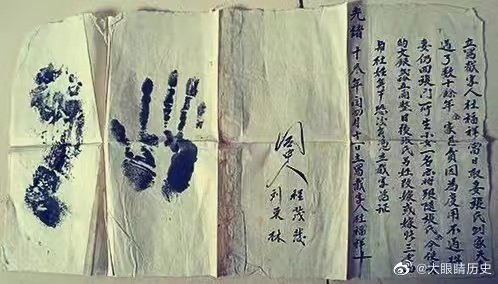
\includegraphics[height=0.36\textwidth,width=0.56\textwidth,viewport=0 0 375 240,clip]{Hand_and_foot-print.png}

\caption*{\hei\hspace{10pt}~

微博网页提供的清代光绪十八年~(公元1892年)~的休书}

\label{Collect_Liu_Wu}

\end{figure}

\includegraphics{.jpeg}

立写截字人杜福祥

当日娶妻张氏到家,夫妻过了数十余年。余家甚贫,因为度用不过,将妻仍回张门,所生小女一名,亦将跟随张氏。余今休妻的(得)文银贰拾伍两整,日后张氏另姓改嫁,或嫁张三、李四,与杜姓无干。恐说无凭,立截字为证。

\begin{flushright}

光绪十八年~闰四月十一日~立写截字人~~杜福祥 ~~(画 ``十字押'') ~~~\\

\large{同中人~程茂发、刘秉林} ~~~~~~~~~~~~~~~ \\

\huge{手模}、\huge{足印} ~~~~~~~~~~~

\end{flushright}

\newpage

\hypertarget{ux6253ux9c7cux6740ux5bb6-ux4e4b-ux8427ux6069}{%

\subsection{\texorpdfstring{打鱼杀家\footnote{ 此戏是《庆顶珠》中的一部分,据有关资料载,原《庆顶珠》全剧有``得宝''、``庆珠''、``比武''、``珠聘''、``打鱼''、``恶讨''、``屈责''、``献珠''、``杀家''、``投亲''、``劫牢''、``珠圆''等场次。一般习惯从``打鱼''演到``杀家'',故称《打鱼杀家》;旧时戏单``鱼''、``渔''混用,亦作``打渔杀家''。据吴小如先生告,1949年后因田汉建议,戏名统一为《打渔杀家》。{514}}

之

萧恩}{打鱼杀家514 之 萧恩}}\label{ux6253ux9c7cux6740ux5bb6-ux4e4b-ux8427ux6069}}

{{[}第一场{]}}

{开船呐!}

{儿啊------}

\setlength{\hangindent}{60pt} {【{\akai 西皮摇板}】父女打鱼在河下,家贫哪怕人笑咱。拉住篷索父把网撒,}

\setlength{\hangindent}{60pt} {【{\akai 西皮散板}】年纪衰迈气力不佳。}

{唉,本当不做这河下生意,你我父女何以度日呀?}

{儿啊,不要啼哭,将船湾在柳荫之下,凉爽凉爽。}

{儿啊,将几尾鲜鱼烹煮好了,少时为父还要饮酒。}

{有人唤我。}

{是哪一位?}

{哦,原来是李贤弟。}

{敢莫要到舟中走走?}

{待我搭了扶手。}

{此位是------?}

{(惊介)这做什么?}

{老了,不中用了。}

{儿啊,出舱来见过二位叔父。}

{小女桂英。}

{一十六岁,痴长啊。}

{且慢,方才打得几尾鲜鱼,就在船头之上,你我弟兄畅快饮一回。}

{儿啊,看酒来。}

{啊,二位贤弟,愚兄有个酒令儿。}

愚兄做的是河下生意,忌的是``干''、``旱''二字。

不敢说罚,要敬酒三杯。

请------

呃,敬你三杯。

哦,待我看来。

诶!做什么的?

问的是哪一家呀?

你来看,就在前面,八字粉墙,合脊门楼,那就是丁$\cdots{}\cdots{}$

诶,哼,放肆!

量他也不敢呐。

请------

哦,又有人唤我。

二位贤弟再饮几杯。

哦,原来是丁郎儿,到此何事啊?

你来看,这几日天旱水浅,鱼不上网。改日有了银钱,送上府去。

哦,是是是。

放他去罢,

教他去罢。

(李俊、倪荣 啊,萧兄为何这等$\cdots{}\cdots{}$。)

他们的人多。

他们的势力大。

这就难讲话了。

本当不做河下生意,怎奈这囊中------唉,惭愧。

哪位贤弟送来?

当面谢过。

有了人家了。

花荣之子,名唤花逢春。

请------

二位贤弟慢走,愚兄不能远送了。

哦,来了。

儿问的是他?

儿啊------

\setlength{\hangindent}{60pt} {【{\akai 西皮摇板}】他本江湖二豪侠,倪荣、李俊就是他。蟒袍、玉带不愿挂,弟兄双双走天涯。}

\setlength{\hangindent}{60pt} {【{\akai 西皮散板}】猛抬头见红日坠落西斜。}

{儿啊,天色不早,我们回去了吧。}

{(kai 正是}: ({\akai 念})父女打鱼在江下,}

{({\akai 念})堪堪不觉红日落,}

{[}第二场{]}

\setlength{\hangindent}{60pt} {【{\akai 西皮快三眼}】昨夜晚吃酒醉和衣而卧,稼场鸡惊醒了梦里南柯。二贤弟在河下相劝与我,他教我把打鱼的事啊一旦丢却。我本当不打鱼啊关门闲坐,怎奈我家贫穷无计奈何。清早起开柴扉乌鸦叫过,飞过来叫过去【{\footnotesize 转}{\akai 西皮二六}】却是为何。将身儿来至在草堂内坐,桂英儿取茶来为父解渴。}

{不教儿渔家打扮,怎么偏偏要渔家打扮?}

{呃------不听父言,就为不孝哇。}

{这便才是!}

{是哪个?}

{你们是哪里来的?}

{哦,原来是丁府上的教师爷。}

{哼!}

{做什么来了?}

{这几日天旱水浅,鱼不上网。改日有钱,送上府去,何必你来!}

{旁人来了无有,教师爷你来了么,}

{哼哼,越发的无有了!}

{朝廷王法,要它何用?}

{哼!}

{哼,尔要锁?}

{当真要锁?}

{果然要锁?}

{如此你就------锁!}

{不教锁。}

{哼!}

{话么,倒是两句好话呀,可惜呀可惜,}

{可惜你二大爷无有工夫啊。}

{尔要讲打?}

{诶呀!老汉幼年间,听说打架,如同小孩子穿新鞋、过新年的一般;如今呐------老了,打不动了啊!}

{尔当真要打?}

{果然要打?!}

{娃娃!待老汉将衣帽留在家中,打个样儿与你们见识见识。}

\setlength{\hangindent}{60pt} {【{\akai 西皮导板}】听一言不由我七窍冒火,}

\setlength{\hangindent}{60pt} {【{\akai 西皮摇板}】不由我年迈人咬碎牙车}\footnote{ 据樊百乐君告知,刘曾复先生强调,``牙车''是``牙床''的意思。吴小如先生曾撰文指出,天津的王庾生先生此句唱作``这才是闭门坐平地生波''。{515}}{。江湖上叫萧恩不才是我,}

\setlength{\hangindent}{60pt} {【{\akai 西皮摇板}】大战场、小战场见过许多。爷本是出山虎独自一个,}

\setlength{\hangindent}{60pt} {【{\akai 西皮摇板}】尔好比看家犬一群一窝。你本是奴下奴敢来欺我。}

{慢说是三``羊头'',就是尔这三``狗头'',二大爷何惧!}

{你是丁府上的教师爷?}

{你好本领呐!老汉要领教领教。}

{一定要领教。}

{这是大十八般武艺?}

{这小十八样兵器?}

{这拳脚是?}

{软硬功夫?}

{呃,这叫什么?}

{不好哇。}

{这叫什么?}

{呃,不好。}

{呃,越发的不好啊。}

{方才撞了老汉三``羊头'',如今我要打你三拳头,放你过去。}

{哪里有功夫。}

{着打!}

{着打!}

{打得好,只恐打出祸来了!}

{那贼回去,定不甘休。待为父赶至县衙,抢他一个原告!}

{不要儿管,取为父的衣帽过来。}

{好好看守门户,为父去去就来。}\footnote{ 陈超老师注: 刘曾复先生曾说明: 此处萧恩\textless{}\!{\bfseries\akai 扫头}\!\textgreater{}下场,不踢大带: 出门,褶子倒手,右手向上一指,弹髯下。这个\textless{}\!{\bfseries\akai 扫头}\!\textgreater{}扫的是一个``对儿'',``闭门家中坐,祸从天上来'',因此这一指表示``祸从天上来''。{516}}

{[}第三场{]}

{(萧桂英

\setlength{\hangindent}{60pt}{ 【{\akai 西皮散板}】老爹爹清晨出前去出首,)}\footnote{ 刘曾复先生为樊百乐君说《审刺客》一戏时,顺便说了``萧恩挨打''部分的内容。{517}} }

{(众\hspace{40pt}~

({\akai 内})一十!)}

{(萧桂英 【{\akai 西皮散板}】倒叫我桂英儿挂在心头。)}

{(众\hspace{40pt}~

({\akai 内})二十!)}

{(萧桂英 【{\akai 西皮散板}】将身儿来至在草堂门口,)}

{(众\hspace{40pt}~

({\akai 内})三十!)}

{(萧桂英 【{\akai 西皮散板}】只等得爹爹回细问根由。)}

{(众\hspace{40pt}~

({\akai 内})四十打完!)}

{(吕子秋 ({\akai 内})赶下堂去!)}

{好贼!}

\setlength{\hangindent}{60pt} {【{\akai 西皮散板}】恼恨那吕子秋为官不正,仗势力欺压我受苦的良民呐。上堂来他那里一言不问,责打我四十板呐赶出了头门。}

\setlength{\hangindent}{60pt} {【{\akai 西皮散板}】我这里咬牙关忙往家奔,叫一声桂英儿你快来开门呐。}

{为父上得堂去,那贼一言不问,将为父重责。}

{这还不算受屈。他教为父连夜过江与那老贼赔礼,那才算受屈呢。}

{哎呀------我恨不得飞过江去,我就杀$\cdots{}\cdots{}$}

{我要杀贼的满门,方消我心头之恨!}

{小小年纪,懂得什么?!不用多管,取为父衣帽、戒刀过来。}

{不用儿管,快些取来。}

{为父去也。}

{何事?}

{小小年纪,去之无益。}

{有此胆量?}

{快将儿的衣服、兵刃收拾好了。}

{壮胆量也是好的。}

{走哇$\cdots{}\cdots{}$}

{做什么?}

{这门么,关也罢,不关也罢呀。}

{又做什么?}

{唉!门都不要了,还要什么家具呀?}

{唉,不明白的冤家呀,呃$\cdots{}\cdots{}$(哭介)}

{不要啼哭,随为父的走哇。}

{儿啊,此番前去,教儿骂,儿就骂,教儿杀,儿就杀,不要害怕。}

{走哇。}

{儿啊,夜晚行船,比不得白日,儿要掌稳了舵!}

\setlength{\hangindent}{60pt} {【{\akai 西皮快板}】这件事不由我心头冒火,今夜晚过江去将他杀却。恨不得插双翅江河越过,}

\setlength{\hangindent}{60pt} {【{\akai 西皮散板}】我的儿因何故放了篷索。}

{杀人还有什么假的不成?}

{呀呸!为父在家中不教儿前来,儿是偏偏地要来。这船行半江之中,儿又要回去------也罢!待为父拨转船头,送儿回去。}

{\textless{}哭头\textgreater{}啊,桂英,我的儿呀!}

{少时还在此处上船,儿记下了?}

{儿啊,庆顶珠}\footnote{ 吴小如先生告,萧恩对萧桂英提及``庆顶珠''时,念白作``聘礼珠子'',``庆顶珠''作戏名。{518}}{可在身旁?}

{此番前去,倘有不测,儿自带庆顶珠逃往花家去吧。}

{我么------儿就不用管了哇。}

{不要啼哭,随我走哇。}

{来此已是。}

{且慢。}

{收拾好了。}

{有人么?走出一个来呀。}

{过府赔罪来了。}

{哼!}

{请了。}

{我来问你: 这鱼税银子,可有圣上旨意?}

{户部公文?}

{凭着何来?}

{敢是那吕子秋?!}

{哼!}

\setlength{\hangindent}{60pt} {【{\akai 西皮摇板}】这税银我不纳是我的本分,你不该差人役打上我门。}

{儿啊,骂呀!}

{且慢,我父女有好心献上。}

{打鱼之时,得来一宗宝贝,名唤庆顶珠。}

{这$\cdots{}\cdots{}$耳目甚多。}

{看刀!}

{儿啊,随为父的杀呀!}

\newpage

\hypertarget{ux7843ux7802ux75e3-ux4e4b-ux97e9ux5ef7ux51e4ux8c2dux6d3e}{%

\subsection{硃砂痣 之

韩廷凤(谭派)}\label{ux7843ux7802ux75e3-ux4e4b-ux97e9ux5ef7ux51e4ux8c2dux6d3e}}

{{[}第一场{]}}

{唉!}

\setlength{\hangindent}{60pt} {【{\akai 二黄摇板}】为续弦前后厅灯光明亮,梦不想今夜晚再做新郎。}

{抬上堂来({\akai 或}: }搭上堂来)\footnote{ 以下括号中的念白据吴焕老师整理的剧本(经刘曾复先生审订)添加。{519}}{。}

{每人赏银二分({\akai 或}: }每人赏钱四个){。}

{带他们下面用饭。}

{待我观看一回。}

\setlength{\hangindent}{60pt} {【{\akai 二黄慢板}】我这里借灯光用目观望,我看她({\akai 或}: 只见她)与前妻一样风光。}

\setlength{\hangindent}{60pt} {【{\akai 二黄慢板}】为什么({\akai 或}: 因何故)皱眉间泪带面上({\akai 或}: 泪带脸上),莫不是嫌年迈难配鸾凰。}

\setlength{\hangindent}{60pt} {【{\akai 二黄慢板}】要穿衣锦绣衫任你选样,}

\setlength{\hangindent}{60pt} {【{\akai 二黄慢板}】要用饭现有那谷米陈仓。}

\setlength{\hangindent}{60pt} {【{\akai 二黄慢板}】这不是那不是难以猜想,尊娘行({\akai 或}: 问娘行)因何事珠泪汪汪,为的是哪桩,你何妨({\akai 或}: 又何妨)细说端详?}

\setlength{\hangindent}{60pt} {【{\akai 二黄摇板}】听她言这婚姻({\akai 或}: 好一似)冰结霜降,一时里惹动我烦恼愁肠。看起来断不可此事勾当,自情愿伴孤灯独守空房。}

{韩福过来。}

{命你同媒婆送这位大娘子回去,对他丈夫言讲({\akai 或}: 与他丈夫言讲): 前番(那)一百两银子不要,再送他一百两银子,教他好好将养疾病,将大娘子送回,成全他夫妻恩义。就此去罢。}

{啊大娘子,还有这婚书呢。}

{唉,就在灯前焚化了罢。}

\setlength{\hangindent}{60pt} {【{\akai 二黄摇板}】伊言道她丈夫病卧床上,没奈何卖妻子暂度时光。将自己比旁人俱是({\akai 或}: 皆是)一样,我岂肯拆散他恩爱鸳鸯。({\akai 或}: 善与恶自有那天理昭彰。)}

{{[}第二场{]}}

\setlength{\hangindent}{60pt} {【{\akai 二黄摇板}\footnote{ 据吴焕老师整理的剧本注: 汪派在``想当年''前面还有两句,词句是``劝世人一个个须要学好,皆因是自有那天理昭彰。''{520}}{】想当年为太守何等荣耀,遇兵荒妻和子无有下梢。多亏了陈太尉将我来保,才能得归田园自在逍遥。}

\setlength{\hangindent}{60pt} {【{\akai 二黄摇板}】忙迫中呃挽定了把礼还到,一时里好教我难解根苗。}

{呜,你不是昨晚送回去的大娘子么?}

{既然将你送回,你又来则甚呐?}

{哦,(原来是)吴相公来了。}

{哎呀,请坐请坐。}

{呃,还有话讲啊。}

{(有话叙谈,}哪有不坐之理,请坐请坐。{)}

{啊大娘子,你也坐下。}

{啊吴相公,昨日听得大娘子说到家中一番苦楚,甚是凄惨。相公有恙在身,改日再来叙谈,为何带病前来?({\akai 或}: 大相公,昨日听得大娘子说到家中一番苦楚。相公你有病在床,病体好了,再来不迟。)}

{哦,你见了银子,出了一身的通汗,这病就好了么?}

{哎呀呀,吴相公啊,看将起来,这银子啊,是好物件!}

\setlength{\hangindent}{60pt} {【{\akai 二黄碰板垛板}】我救你的急,救你的难,救你的贫困;全尔的节,全尔的义,全尔的婚呐姻。纵有妻不生子前生造定,我岂肯拆婚姻}\footnote{ 此处刘曾复先生说戏录音近似``错婚姻'',吴小如先生从夏山楼主学的是``拆婚姻'',此处从吴小如先生。李楠君认为,此处系刘曾复先生将``拆''字按上口字处理。{521}}{落下了骂名。}

{啊,啊,呵呵呵哈哈哈$\cdots{}\cdots{}$(笑介)}

{请坐请坐。}

{哎呀呀吴相公啊,我当日也是恩爱夫妻,只因兵荒马乱,中途失散,却无子嗣。若有一子传宗接代,我也就不续弦再娶的了哇。}

{这$\cdots{}\cdots{}$子孙前世所修,再续么,也就不必了。({\akai 或}: }子孙之事,前生所修。再娶么,唉,也就不必了。{)}

{言得极是,只是本处孩儿多有不便呐。}

{本当如此,奈无机会。}

{这只好凭天机、遇时宜了。}

{吴相公慢些走啊!}

\setlength{\hangindent}{60pt} {【{\akai 二黄摇板}】他夫妻进门来双双拜倒({\akai 或}: 双双跪倒),口声声叫恩人泪似呃雨抛。非是我用银钱假意行好哇,韩廷凤全仁义一片心苗。}

{{[}第三场{]}}

\setlength{\hangindent}{60pt} {【四平调】叹光阴去不归无限烦闷,不觉已老两鬓如银。读古书难解我心头烦闷,饮香醪怎畅我衷肠凄清。}

{哦,你是吴相公,呃,请坐请坐。}

{你往成都收取账目,呃,必定是发了财了哇。({\akai 或}: }闻你往成都,收取账目,一定发财的了。{)}

{请便。}

{哦,这是何人?}

{哦,罢了(罢了),一旁坐下。}

{呃,不妨不妨,只管地坐下。}

{呵呵呵哈哈哈$\cdots{}\cdots{}$(笑介)}

{啊吴相公,你看这小小的孩童,呃,也(很)知大体呀。}

{是啊,小孩子原要(他)爹娘教导哇。}

{啊吴相公,你买他前来,还是为子啊,还是为仆呢?}

{哦,这等说来({\akai 或}: }如此说来){,是送与我的?}

{哎呀呀吴相公啊,你真是({\akai 或}: }你真乃){信实人也。}

\setlength{\hangindent}{60pt} {【四平调】吴官人你真真言而有信,你与我谋后代不惜辛勤。感谢你这好意情深义尽,\textless{}行弦\textgreater{}}

{吴大哥,你请来上坐。({\akai 或}: }这边坐,这边坐。{)}

{请坐,请坐。}

\setlength{\hangindent}{60pt} {【四平调】退一日自当另有条陈。}

{呵呵哈哈哈$\cdots{}\cdots{}$(笑介)}

{哎呀吴官人呐,我如今有了儿子就不愁了。}

{是啊,吴官人离家日久,我也不便相留({\akai 或}: }不便强留{),改日我父子要登门叩谢。}

{儿啊,送过你吴大爷。}

{(啊,吴官人何事?)}

{请来吃酒,请来吃酒。}

{啊$\cdots{}\cdots{}$呃,吴官人,请转请转。}

{改日我父子,呃,要登门再谢。}

{呃一定要去,一定要去。}

{啊$\cdots{}\cdots{}$呃,无有了,请便请便。({\akai 或}: }吴官人,请呐请呐。{)}

{哦------哈哈哈$\cdots{}\cdots{}$(笑介)}

{儿啊,随为父的进来。}

{一旁坐下,待我细看一回({\akai 或}: 待我}细观一回{)。}

\setlength{\hangindent}{60pt} {【{\akai 二黄原板}】我的儿须从容端然坐定,看形象并非是平等之人。细观他各部位五官端正,这两鬓齐开朗目秀眉清。儿在家可读过圣贤书本,一一地对为父细说分明。}

\setlength{\hangindent}{60pt} {【{\akai 二黄原板}】他说话有分寸智慧聪明,倒像个宦门后不差毫分。可记得是何年月日生辰,说出来将八字细与儿评。}

\setlength{\hangindent}{60pt} {【{\akai 二黄原板}】这小娃言语中隐藏暗景,再问他亲父母便知真情。儿父母年多少在不在,因何故图银钱卖与他人。}

{儿今年多大年纪了({\akai 或}: }儿今年几岁了{) ?}

{儿父?}

{死了五载。}

{儿母?}

{七旬有余。}

{(惊介)儿有一十三岁({\akai 或}: }儿才一十三岁{)。}

{(惊介)嗯$\cdots{}\cdots{}$}

\setlength{\hangindent}{60pt} {【{\akai 二黄原板}】这其间又盘出}\footnote{ 吴焕老师整理的剧本记作``又攀出''。{522}}{奇情种种,哪有个花甲年又产娇生。}

{儿啊------}

\setlength{\hangindent}{60pt} {【{\akai 二黄原板}】必然是那老娘将儿蒙混,这内中另有个生儿的娘亲。}

{哦,儿是捡来的么?}

\setlength{\hangindent}{60pt} {【{\akai 二黄原板}】细盘问这来由日月推论,仔细想当年事越加是真: 宣和年四月里成都调任,行至在青州府路遇贼兵。亲生儿在娘怀无有踪影,实可怜贤德妻命赴幽冥。}

\setlength{\hangindent}{60pt} {【{\akai 二黄散板}】这形象好一似韩门真种,举动间与老夫骨肉有情。我这里取菱花照照相品呐,}

\setlength{\hangindent}{60pt} {【{\akai 二黄散板}】半像我半像妻不差毫分。}

\setlength{\hangindent}{60pt} {【{\akai 二黄散板}】亲生子再相逢三生有幸,这才是天地意弄假成真。}

{不对了,不对了!}

{(韩玉印 怎么不对呢?)}

{我那亲生的孩儿,落生下来,左足心上有硃砂红痣。你无有,不是我的亲生儿子啊。}

{怎么,儿也有?}

{为父的不信呐,待我看来。}

{(唉,儿啊------)}

\setlength{\hangindent}{60pt} {【{\akai 二黄散板}】你是我亲生的儿呀名唤玉印,遇兵荒遭失散十有二春。盼娇儿盼得我身染重病,盼娇儿盼得我昼夜不宁。盼娇儿啊不做官告归故呃井,喂呀我的儿呀,梦不想天保佑枯木哇逢春。}

{你母命丧东平,也曾命人搬尸去了$\cdots{}\cdots{}$哇,呃$\cdots{}\cdots{}$(哭介)}

{言得极是,派人接她前来就是。}

{(kai 正是}: ({\akai 念})北转南来西复东,今朝骨肉又重逢。父子再把菱花照,}

{(儿啊------)}

{({\akai 念})只怕相逢在梦中。}

{哦,不是做梦?}

{玉印,我儿,啊------啊------哈哈哈$\cdots{}\cdots{}$(笑介)}

{随我来。}

\newpage

\hypertarget{ux96c4ux5ddeux5173}{%

\subsection{雄州关}\label{ux96c4ux5ddeux5173}}

{{[}第一场{]}}

{呼延狄\hspace{20pt}~

({\akai 念})百万熊罴犯中原,}

{雷洪切\hspace{20pt}~

({\akai 念})搅乱宋室不安然!}

{达林呈\hspace{20pt}~

({\akai 念})渴饮马上刀头血,}

{季乐芬\hspace{20pt}~

({\akai 念})嘿!饥饿人头当饭餐!}

{众\hspace{40pt}~

俺------}

{呼延狄\hspace{20pt}~

金邦大将军呼延狄是也!}

{雷洪切\hspace{20pt}~

金邦副将军雷洪切是也!}

{达林呈\hspace{20pt}~

金邦左先锋达林呈是也!}

{季乐芬\hspace{20pt}~

金邦右先锋季乐芬是也!}

{萨里哈\hspace{20pt}~

前营骁骑大将军萨里哈是也!}

{耶律浑\hspace{20pt}~

后营骁骑大将军耶律浑是也!}

{提尔雄\hspace{20pt}~

左营压队大将军提尔雄是也!}

{虎骨达\hspace{20pt}~

右营护卫大将军虎骨达是也!}

{呼延狄\hspace{20pt}~

列位将军请了------}

{众\hspace{40pt}~

请了!}

{呼延狄

你我奉了狼主之命,随定四太子,领兵夺取宋室天下,兵到即克。也是宋王气数当尽了。}

{众\hspace{40pt}~

着啊!}

{呼延狄\hspace{20pt}~

这些蛮子怎能苦争恶战,这也是我家狼主洪福齐天也!}

{众

听觱篥}\footnote{ 段公平君注: 觱篥,又作``筚篥'',竹管乐器,源于西域,类似``胡笳''。即俗称``牛角觱篥''者,番邦号角。{523}}{一声响,太子升帐,你我两厢伺候。请------}

{金兀朮

\textless{}点绛唇\textgreater{}军营号响}\footnote{ 段公平君建议作``各路豪强''。{524}}{,威武雄壮;中军帐,排列刀枪,杀气呃------}

{众\hspace{40pt}~

参见殿下!}

{金兀朮\hspace{20pt}~

站立两厢!}

{金兀朮

({\akai 念})杀气腾腾满乾坤,哀声处处震天庭。宋王失政宠奸佞,锦绣江山一旦倾。}

{金兀朮

孤,北番大金邦女真国老王殿下四太子、昌平王、御营总兵完颜兀朮。今有宋主无道,宠信奸臣。内奸童贯封为广阳王}\footnote{ 此处从《传统剧目汇编》,童贯封``广阳王''。{525}}{之职。是他前者有密书到孤父王驾下,约定我国兴兵夺取他家社稷。有他以为内应,这宋室天下岂不是唾手而得。自兴兵以来,战无不胜,攻无不取。前日又破了潞安州,守将陆登自刎身亡,甚是悲惨。前面乃是雄州关,守将韩世忠。此人乃是忠勇之士,孤家不忍逼迫于他。意欲招他归顺,助孤一臂之力,何愁大事不成。}

{金兀朮\hspace{20pt}~

众番儿!}

{众\hspace{40pt}~

有!}

{金兀朮\hspace{20pt}~

此番兴兵行至雄州关,不可杀掠黎民,违令者斩!}

{众\hspace{40pt}~

啊!}

{金兀朮\hspace{20pt}~

由此发动人马!}

{{[}第二场{]}}

{探子\hspace{30pt}~

马来。}

{探子

({\akai 念})短甲随身衲袄齐,肩上横担令字旗。年年岁岁领皇赏。一马冲至军队里。}

{探子

俺,韩元帅麾下能行探子是也。奉了元帅将令,着俺四路哨探。今有圣上差孙浩督兵前来剿灭金邦,已至三山口。不免飞骑报韩元帅知道!就此马上加鞭。}

{{[}第三场{]}}

{韩世忠

\setlength{\hangindent}{60pt}{ 【{\akai 西皮三眼}】为金兵急得我心神不定,盼救}兵望眼穿昼夜不宁。陆元帅尽了忠自刎丧命,只一子失陷在万马军营。好教人止不住啊 }

【{\footnotesize 转}{\akai {西皮二六}】腮边泪滚,可叹他夫妻们饮恨幽冥。行公文\footnote{ 夏行涛君建议作``赍公文''。{526}}求圣上遣将助阵,因何故十数日渺无回音。在二堂思无计心呃中忧闷,我父子只恐怕难退雄兵。

中军\hspace{30pt}~

({\akai 念})探马如飞急,叩禀元帅知。

中军\hspace{30pt}~

启元帅: 探马求见。

韩世忠\hspace{20pt}~

吩咐开门!

中军\hspace{30pt}~

开门!

众\hspace{40pt}~

啊!

韩世忠\hspace{20pt}~

{({\akai 念})}探马报音信,升帐问分明。

韩世忠\hspace{20pt}~

传探马。

中军\hspace{30pt}~

元帅有令: 探马进见。

探马\hspace{30pt}~

报------告进。

探马\hspace{30pt}~

帅爷在上,探马叩头。

韩世忠\hspace{20pt}~

打听哪路军情,起来快些讲。

探马\hspace{30pt}~

啊,帅爷听禀: 

探马

({\akai 念})一马哨探似流星,朝中差来孙总兵。十万人马到疆界,禀报元帅得知情。

韩世忠\hspace{20pt}~

朝中无有什么姓孙的呀!

探马\hspace{30pt}~

在元帅帐下当过副将的。

韩世忠\hspace{20pt}~

哦------敢是孙浩?!

探马\hspace{30pt}~

正是。

韩世忠\hspace{20pt}~

赏尔金牌一面,再去打探。

探马\hspace{30pt}~

得令!

韩世忠

且住!想那孙浩,在某帐下曾为副将。只因犯我将令,将他捆打,是他逃至京中,投在{广阳}府内,做了随侍。今番奉旨督兵前来,焉有不接之理。

韩世忠\hspace{20pt}~

中军!

中军\hspace{30pt}~

有!

韩世忠\hspace{20pt}~

传众将进帐。

中军\hspace{30pt}~

众将进帐呃!

{四将}\hspace{30pt}~

({\akai 内})来也!

{四将}

({\akai 念})元帅传军令,将士共趋迎\footnote{ 夏行涛君建议作``躬躯迎''。{527}}。

{四将}\hspace{30pt}~

参见元帅。

韩世忠\hspace{20pt}~

众位将军少礼!

{四将}\hspace{30pt}~

啊!

{四将}\hspace{30pt}~

传末将等进帐,有何军情议论?

韩世忠\hspace{20pt}~

圣上命孙浩督兵前来,征剿金人,已到三山口。命你等前去迎接。

{四将}\hspace{30pt}~

啊元帅,那孙浩若问: 你家元帅为何不来。我等怎样回答?

韩世忠

你等就说: 我家元帅因金兵犯境,城内空虚,不敢擅离汛地,故命我等前来迎接。

{四将}\hspace{30pt}~

那孙浩缘何授得此职?

韩世忠\hspace{20pt}~

唉!你等不知他的来历,听我令下: 

{韩世忠

\setlength{\hangindent}{60pt}{ 【{\akai 西皮}原板}】韩世忠坐宝帐传言发令,叫一声众将官细听详情: 那孙浩平日间行为不正,犯军令责罚他不能徇情呃。逃到了京师地{广阳}府进,童太尉听谗言懵懂圣君。迎接他务须要言语谨慎, }

{韩世忠\hspace{20pt}~

\setlength{\hangindent}{60pt}{ 【{\akai 西皮摇板}】防贼子寻仇起暗箭伤人。 }

{四将\hspace{30pt}~

得令!}

{四将\hspace{30pt}~

\setlength{\hangindent}{60pt}{ 【{\akai 西皮摇板}】韩元帅忠义士谁人不敬,何惧那孙浩贼势利小人。} }

{韩世忠

\setlength{\hangindent}{60pt}{ 【{\akai 西皮摇板}】大宋朝八代君徽宗失政,贪酒色戮忠良信宠谗臣。恨蔡京与童贯伤害民命,惹得那四路里齐动刀兵。金兀朮领人马抢夺州郡,逼元戎劳将士苦及黎民。众将官退宝帐各归管汛,} }

{韩世忠\hspace{20pt}~

\setlength{\hangindent}{60pt}{ 【{\akai 西皮摇板}】且等候四将回再定计行。} }

{{[}第四场{]}}

{孙浩

\textless{}点绛唇\textgreater{}奉旨领雄兵,蟒罗袍,不愧先人;定斩世忠消吾恨,还报他痛打军刑。}

{孙浩}

({\akai 念}){胸怀巧诈极聪明,不近贵人怎升腾?只道一生空劳力,运至时来命通亨。}

{孙浩

某,孙浩,塞北人也。昔在韩世忠麾下以为步军,只因不守军规,专意花酒情浓。抢得一有夫之妇作乐,不想韩世忠便要将俺斩首。是俺推在步兵列名身上,彼时将那步兵斩首号令。又道俺带领无方,将俺捆打,削去头领,赶出不用。俺又羞又恼,一怒奔至京中。恰遇童太尉朝罢而归,是俺闯了他的禁道,将我拿到府中拷问。俺将韩世忠打革之事从头诉说一遍,不想童太尉与韩世忠是旧有仇恨,听了此言,便把俺留在府呃中。因俺善于奉承,是他心中欢喜,想要重用于俺。如今金兀朮兴兵犯界,破了无数城池。眼看要到雄州,那韩世忠本章进京,求兵添将。童太尉奏上一本,命俺提兵前来,剿灭番贼。若是得胜,道韩世忠贪生怕死;若是损兵,便道韩世忠按兵不动。慢说是一个韩世忠,就是百个,也教他有死无生。看前面已是三山口,众将,催动人马!}

{孙浩\hspace{30pt}~

\setlength{\hangindent}{60pt}{ 【{\akai 西皮导板}】见旌旗空中飘人声喧震,} }

{孙浩

\setlength{\hangindent}{60pt}{ 【{\akai 西皮原板}】抖起}了万丈尘沸沸腾腾。曾记得到京都那般光景,岂料我今日里督领雄兵。韩世忠好比那儿童之分,怎知晓暗中刀要你残生。咱料他如南柯梦魂未醒, }

{孙浩\hspace{30pt}~

\setlength{\hangindent}{60pt}{ 【{\akai 西皮摇板}】绑云阳一命倾才晓前情。 }

{孙浩

前道}\footnote{ 段公平君建议作``前导''。{528}}{为何不行?}

{四将\hspace{30pt}~

雄州关总戎麾下四营将校迎接总爷。}

{众\hspace{40pt}~

雄州关总戎麾下四营将校迎接总爷。}

{孙浩\hspace{30pt}~

传。}

{众\hspace{40pt}~

传。}

{四将\hspace{30pt}~

雄州关四营将校迎接总爷}

{孙浩\hspace{30pt}~

你家主帅有多大的官儿,怎么不来迎接本镇。}

{四将

启禀总爷: 主帅为金兵临界,关内空虚,不敢擅离汛地,故而命末将等前来迎接总爷。}

{孙浩

哼------你住了!本镇钦奉圣命,广阳王钧旨,领兵剿贼,你们主帅也不看在眼内,本当将尔等捆打------}

{四将\hspace{30pt}~

总爷开恩。}

{孙浩\hspace{30pt}~

也罢!待本镇破了金兵回来,再与你主帅辩理。}

{孙浩\hspace{30pt}~

来呀,乱棍逐出!}

{孙浩\hspace{30pt}~

催------军!}

{孙浩

\setlength{\hangindent}{60pt}{ 【{\akai 西皮摇板}】定教他主帅们无处逃奔,少不得斩尔等碎尸粉身。叫众将越过了飞龙奇岭,扫灭了番邦贼奏达捷音。} }

{{[}第五场{]}}

{韩世忠

\setlength{\hangindent}{60pt}{ 【{\akai 西皮摇板}】命四将接孙浩渺无音信,倒教我背地里暗自思忖呐。必然他要报那从先的仇恨,可惜我空费了一片精神。} }

{四将\hspace{30pt}~

\setlength{\hangindent}{60pt}{ 【{\akai 西皮摇板}】贼孙浩忒无礼令人可恨,全不念数年间共事同营。} }

{四将\hspace{30pt}~

参见元帅!}

{韩世忠\hspace{20pt}~

你们回来了。}

{四将\hspace{30pt}~

回来了。}

{韩世忠\hspace{20pt}~

迎接孙浩他可曾讲些什么?}

{四将\hspace{30pt}~

末将等奉令迎接孙浩,那厮言道: 你家主帅为何不来?}

{韩世忠\hspace{20pt}~

你等怎生回答?}

{四将

末将言道: 金兵临界,城内空虚,不敢擅离汛地,故命我等前来迎接}

{韩世忠\hspace{20pt}~

那厮如何言道?}

{四将

那厮言道: 本镇钦奉圣命,广阳王钧旨,领兵剿贼,你主帅有多大的官儿,不来迎接本镇。本当将尔捆绑------待等破了金兵回来,再与你主帅辩理。说罢此言,呃,将我等乱棍,呵,逐出来了。}

{韩世忠\hspace{20pt}~

小人得志,以致如此。}

{探子\hspace{30pt}~

报!启禀元帅: 孙浩越过飞龙岭,迎战金兵去了。}

{韩世忠\hspace{20pt}~

再探!}

{韩世忠

且住!我想孙浩越过飞龙岭与金兵迎战,倘有差池本帅难逃罪责。}

{韩世忠\hspace{20pt}~

来,传彦直进帐。}

{中军\hspace{30pt}~

有请少将军。}

{韩彦直\hspace{20pt}~

来也!}

{韩彦直\hspace{20pt}~

({\akai 念})战国英雄数伍员,一忿扫平楚国兵。}

{韩彦直\hspace{20pt}~

参见父帅。}

{韩世忠\hspace{20pt}~

罢了!坐下。}

{韩彦直\hspace{20pt}~

谢座。唤孩儿进帐,有何吩咐?}

{韩世忠

圣上命孙浩督兵前来,征剿金人,那贼从飞龙岭迎敌去了。命你带领人马,暗地保护,需要小心在意,听为父令下: }

{韩世忠

\setlength{\hangindent}{60pt}{ 【{\akai 西皮摇板}】广阳王点孙浩身当重任,命四将迎接他赶回州城。我的儿领人马暗地接应,钦命官须保护谨慎小心。} }

{韩彦直\hspace{20pt}~

得令!}

{韩彦直

\setlength{\hangindent}{60pt}{ 【{\akai 西皮摇板}】在帐中领将令怎敢迟顿,暗地里保孙浩谨慎殷勤。}\footnote{ 刘曾复先生介绍,此处唱下是程继先的演法,金仲仁的演法是念下。{529}} }

{韩世忠\hspace{20pt}~

众将官,随本帅披挂,催动人马,起兵前往!}

{{[}第六场{]}}

{金兀朮\hspace{20pt}~

马前来的将官,可是韩元帅?}

{孙浩\hspace{30pt}~

逆贼,俺乃童太尉府中的心腹之人,剿贼大将军孙浩是也!}

{金兀朮\hspace{20pt}~

奸贼一党,休要放走之呃!}

{{[}第七场{]}}

{韩彦直

({\akai 念})头戴束发紫金冠,金锁铠甲扣连环。胸怀重瞳英雄胆,宝剑出鞘血未干。}

{韩彦直\hspace{20pt}~

俺,韩彦直。奉了父帅之命,暗地保护孙浩。}

{韩彦直\hspace{20pt}~

众将官!}

{众\hspace{40pt}~

有!}

{韩彦直\hspace{20pt}~

杀上前去!}

{{[}第八场{]}}

{探子\hspace{30pt}~

启元帅: 孙浩落马;少爷杀进番营去了!}

{韩世忠\hspace{20pt}~

再探!}

{韩世忠\hspace{20pt}~

且住!孙浩落马,我儿杀进番营,这还了得!}

{韩世忠\hspace{20pt}~

众将官,}

{众\hspace{40pt}~

有!}

{韩世忠\hspace{20pt}~

奋勇当先!}

{{[}第九场{]}}

{金兀朮

住了,你这小儿,二次杀进番营,倒有些胆量,饶尔不死,通名上来!}

{韩彦直\hspace{20pt}~

听者: 俺乃雄州关总戎之子韩彦直是也。}

{金兀朮\hspace{20pt}~

你就是韩世忠之子么?!}

{韩彦直\hspace{20pt}~

然也。}

{金兀朮\hspace{20pt}~

哎,真乃是将门之子!}

{韩彦直\hspace{20pt}~

呔,番贼通名受死。}

{金兀朮\hspace{20pt}~

孤乃大金邦四太子昌平王兀朮是也。}

{韩彦直\hspace{20pt}~

着打!}

{韩世忠\hspace{20pt}~

彦直,孙浩何在?}

{韩彦直\hspace{20pt}~

被番兵踹为肉泥。}

{韩世忠\hspace{20pt}~

好哇!儿啊,下马来,为父有话言讲。}

{韩彦直\hspace{20pt}~

是。}

{韩世忠\hspace{20pt}~

好奴才!}

{韩世忠

\setlength{\hangindent}{60pt}{ 【{\akai 西皮散板}】为父怎样将儿命,断送孙浩丧番营。金枪刺儿咽喉哽,} }

{韩彦直\hspace{20pt}~

\setlength{\hangindent}{60pt}{ 【{\akai 西皮散板}】要杀孩儿为何情?} }

{韩世忠

大胆畜生,为父可曾}\footnote{ 段公平君建议作``何等''。{530}}{吩咐与你?!那孙浩乃是圣上差来,又是广阳王的保举,教儿小心暗护,竟被番营杀死,倘若圣上闻知,必道为父有按兵不动之罪。哎呀!儿啊!岂不把为父的送在枉死城去?!}

{韩彦直

哎呀,爹爹呀!孩儿奉命暗护孙浩,杀进番营,并无此人。况且儿又不认识于他。}

{韩世忠\hspace{20pt}~

住了!那孙浩乃是领兵元戎,必有旗号,儿也不认得吗?}

{韩彦直

哎呀,爹爹呀!孩儿虽然奉令暗护孙浩,但是万马营中,犹如刀山剑岭,难道教儿束手待死不成?!}

{四将\hspace{30pt}~

元帅,公子之言甚是,还望元帅开恩。}

{韩世忠

也罢,命儿三次杀进番营,杀退番邦便罢,如若不然,定斩尔的首级。}

{韩彦直\hspace{20pt}~

得令呐!呵$\cdots{}\cdots{}$(哭介)}

{韩世忠\hspace{20pt}~

哼!}

{韩世忠\hspace{20pt}~

众将官,直踹番营!}

{{[}第十场{]}}

{金兀朮\hspace{20pt}~

呔,马前来的敢是韩元帅?}

{韩世忠\hspace{20pt}~

然。马前搭话敢是兀朮?}

{金兀朮\hspace{20pt}~

然。}

{韩世忠

兀朮!吾主有何亏负尔等,既破潞安州,又来兵犯吾郡,是何理也?}

{金兀朮

韩元帅,你且停战马,听某一言告禀: 你主贪淫失政,宠信奸佞,忠良遭戮,以致刀兵四起。莫若归顺我邦,得了宋室天下,定是三台鼎鼐之位。元帅上察!}

{韩世忠

兀朮,你韩元帅兵虽少个个勇。你强夺州郡}\footnote{ 夏行涛君建议作``抢夺州郡''。{531}}{,伤害人民,恨不得食尔之肉,还敢多言么?}

{韩世忠

\setlength{\hangindent}{60pt}{ 【{\akai 西皮摇板}】战鼓嗵嗵山岳动}\footnote{ 此处俗作``山摇动''。{532}}{,番邦贼寇敢逞能。扫灭狼烟归大宋,方显男儿是英雄。} }

{金兀朮\hspace{20pt}~

韩元帅。}

{金兀朮

\setlength{\hangindent}{60pt}{ 【{\akai 西皮摇板}】久闻世忠武艺灵}\footnote{ 夏行涛君建议作``有威名''。{533}}{,今日见面果俊英。堂堂仪表非俗品,胜似战国楚伍员。} }

{金兀朮\hspace{20pt}~

韩元帅。}

{金兀朮\hspace{20pt}~

\setlength{\hangindent}{60pt}{ 【{\akai 西皮摇板}】你若马前来归顺,孤家与你皇兄称。} }

{韩世忠\hspace{20pt}~

住了!}

{韩世忠

\setlength{\hangindent}{60pt}{ 【{\akai 西皮摇板}】兀朮开言真堪恨,气得本帅怒上升。收兵回马保众命,不然杀尔草寇平。} }

{{[}第十一场{]}}

{韩世忠\hspace{20pt}~

参见圣上!}

{童贯

韩世忠!按兵不动,陷害朝廷命官,有降顺金邦之意!来啊!打入囚车!}

{韩世忠\hspace{20pt}~

唉呀!}

{探子\hspace{30pt}~

报!金兵四面围困。}

{童贯\hspace{30pt}~

再探!}

{童贯\hspace{30pt}~

唉呀!}

{童贯\hspace{30pt}~

也罢!韩世忠,命你杀退金兵,将功折罪呀!}

{韩世忠\hspace{20pt}~

奋勇当先!}

{金兀朮\hspace{20pt}~

好小子呃!}

{韩世忠\hspace{20pt}~

追呃!}

{韩世忠\hspace{20pt}~

哈哈,哈哈,啊------呵呵哈哈哈$\cdots{}\cdots{}$(笑介)}

{韩世忠\hspace{20pt}~

收兵呐!}

\newpage

\hypertarget{ux9547ux6f6dux5dde-ux4e4b-ux5cb3ux98deux6768ux749f}{%

\subsection{镇潭州 之

岳飞、杨璟}\label{ux9547ux6f6dux5dde-ux4e4b-ux5cb3ux98deux6768ux749f}}

{{[}第一场{]}}

{岳飞

\textless{}点绛唇\textgreater{}报国精忠,虎啸龙吟;迎二圣,扫荡烟尘,保主锦绣春。}

{岳飞

({\akai 念})旌旗招展出禁城,武将心思汗马勋。剖心要尽凌云志,迎回二圣方称心。}

{岳飞

本帅,姓岳名飞字鹏举,宋室驾前为臣。只因奸佞当道,张邦昌陷二圣于沙漠,坐井观天。是我退归林下;今蒙太后二次诏宣,官拜天下都招讨、兵马大元帅;后宫娘娘恩赐五色锦旗,亲绣``精忠报国''。}

{岳飞

本帅亲承王命,统领六师,扫荡烟尘,恢复河山。今乃黄道吉日,正好兴兵。众位贤弟!}

{岳飞\hspace{30pt}~

人马可齐?}

{岳飞\hspace{30pt}~

香案伺候!}

{岳飞

祝告: ({\akai 念})山川社稷、万里旗纛尊神: 信官岳飞,今奉圣命,扫荡九龙山杨再兴、长沙王罗延庆、洞庭湖水贼杨幺等。但愿此行,旗开得胜!}\footnote{ {据陈超老师介绍: }奠酒上丑司仪,圆纱白四喜青褶子(不穿官衣),上三炷香、三叩首。很特别。{534}}

{岳飞\hspace{30pt}~

打道出府。}\footnote{

``{打道出府}''一句,陈超老师从刘曾复先生学的是``{撤去香案}''。省事。{535}}

{岳飞\hspace{30pt}~

牛皋听令。}

{岳飞\hspace{30pt}~

命你去到潭州晓谕节度使,命他高垒城郭,本帅大兵随后就到。}

{岳飞\hspace{30pt}~

转来。}

{岳飞\hspace{30pt}~

岳云听令。}

{岳飞\hspace{30pt}~

解押粮草}

{岳飞\hspace{30pt}~

张宪听令。}

{岳飞\hspace{30pt}~

催运粮草}

{岳飞}\hspace{30pt}~

张保{听令。}

{岳飞\hspace{30pt}~

命你以为总督粮官。}

{岳飞\hspace{30pt}~

吉青听令。}

{岳飞\hspace{30pt}~

随营护卫。}

{岳飞\hspace{30pt}~

施全听令。}

{岳飞

命你总督三军。}传令下去,众将一路之上,不可马踏青苗,扰害百姓,违令者斩!

{岳飞}\hspace{30pt}~

就此起兵潭州。

{{[}第二场{]}}

{岳飞\hspace{30pt}~

哦,恩师!}

{岳飞\hspace{30pt}~

不敢,恩师请!}

{岳飞\hspace{30pt}~

门生放肆。}

{岳飞\hspace{30pt}~

门生有何德能,敢劳恩师迎接十里之外?}

{岳飞\hspace{30pt}~

惶恐啊惶恐!}

{岳飞\hspace{30pt}~

我命牛皋前来,为何不见?}

{岳飞\hspace{30pt}~

哦,牛皋至此,未憩鞍马,径自立功去了?}

{岳飞\hspace{30pt}~

嗯------想他此去,必然是大败而归。}

{岳飞\hspace{30pt}~

贤弟,你与敌人交战,胜负如何?}

{岳飞\hspace{30pt}~

怎么样?}

{岳飞\hspace{30pt}~

可曾问过敌人的名姓?}

{岳飞

呃------你跟随愚兄出兵多年,还是这样粗鲁,倘若得胜而归,教愚兄怎上功劳簿。}

{岳飞\hspace{30pt}~

敢是那杨再兴?}

{岳飞\hspace{30pt}~

此人英勇无敌,你岂是他人对手,待本帅亲自会他。}

{岳飞

众位贤弟!有所不知,想那杨再兴,乃是将门之子,名门之后,武艺高强,本帅意欲,将他收留帐下,做一膀臂。今日出马,非比寻常,众将只许观阵,不许助战,违令者斩!}

{岳飞\hspace{30pt}~

恩师不必拦阻,待门生先见一阵。}

{岳飞\hspace{30pt}~

就烦恩师谨守城池。}

{岳飞\hspace{30pt}~

众将官,带马迎敌者。}

{岳飞\hspace{30pt}~

杨将军,别来无恙!}

{岳飞\hspace{30pt}~

杨将军,想那年在汴梁小校场,会过一面,难道将军你就忘怀了?}

{岳飞\hspace{30pt}~

然也。}

{岳飞

杨将军,想你乃是将门之子,忠良之后,因甚事失身落草,岂不玷辱杨氏祖先?听本帅相劝,归顺皇朝,共灭金寇,不失封侯之位,将军三思。}

{岳飞\hspace{30pt}~

住口!好言相劝,执意不听,少时擒在马前,悔之晚矣!}

{岳飞\hspace{30pt}~

决一胜负。}

{岳飞\hspace{30pt}~

这个$\cdots{}\cdots{}$杨将军,俺若不胜,情愿将潭州奉让。}

{岳飞

杨将军,你我今日交战,非比寻常,必须一对一个;两下各传将令,众将只许观阵,不许助战,违令者斩。}

{岳飞\hspace{30pt}~

军令不严非为丈夫也。}

{岳飞\hspace{30pt}~

\textless{}叫头\textgreater{}众将官!}

{岳飞\hspace{30pt}~

只许观阵,不许助战,违令者斩!}

{岳飞\hspace{30pt}~

\setlength{\hangindent}{60pt}{ 【{\akai 西皮小导板}】叫三军与爷战鼓操,} }

{岳飞

\setlength{\hangindent}{60pt}{ 【{\akai 西皮快板}】马前闪出一英豪。杨家世代把国保,因何埋名在山巢。劝你马前归顺好,封妻荫子永在朝。} }

(上手(岳飞)大边,一扯两扯,幺二三往外把盖下手(杨再兴)枪左转身(下手右转身)到里边打一个腰封、两个腰封,被往里面盖右转身(下手左转身)到外边,接一个腰封、两个腰封,把盖撤枪,撤右脚斜向上场门,上左脚刺在上场边里面的下手左右两马腿,左刺耳\footnote{ 陈超老师注: 此处{老生左刺耳是两枪},{小生是刺一枪}。刘先生当初稿里写了两枪,《戏曲艺术》发表时漏排。要是一枪小生倒不过抢来,老生刺两枪,小生枪鐏接一个,剜花,枪头接一个。{536}},被下手盖,撤枪撤左腿在下场门边外面接下手两个刺马腿,盖下手左刺耳,搭、拉归里边面外、下手面里,搭、兜转身过到小边,面对过大边的下手掣肘,撤枪两人对脸左右左三个刺马腿,一二三绕、边绕边走从外面过到大边,一二三绕,边绕边走从外面过到小边,下手向内侧刺上手马腿、上手挑起向里刺肚,从里边左转身到外边向外侧刺下手马腿、下手挑起来刺肚,下手直着过到小边,上手接刺肚向右反转身从里边过到大边,二人合身往里一盖两盖,上手手平伸扎下手一枪左转身(下手左手拿枪滑上手扎出的枪、右转身右手掏翎,送到嘴叼翎,枪交右手),上手左手捋胡子、跨右腿、左转身又扎下手一枪(下手右手枪滑上手枪,右转身左手掏翎子),上手转过来扔胡子、枪收回来平托、左手山膀,大边里边站斜向外亮住(下手转过来右手枪剜萝卜、右手伸出、枪头斜向下,左手拿翎横胸前,弓箭步外边站斜向里亮住)\footnote{ 这是刘砚芳介绍的杨小楼的《镇潭州》中岳飞与杨再兴开打的``枪架子''头场的打法。  杨的岳飞学谭鑫培,所用的把子能显出大将风度,马上交锋,彼此较量,稳重沉着,棋逢对手,合乎剧情。  \begin{quote}  陈超老师补注: 杨小楼跟梅兰芳唱过《镇潭州》,也打这套把子,是杨小楼教的。程继先、杨小楼没唱过这出戏,程继先从没搭过杨小楼班,也不单独与杨合作唱戏,只是在窝窝头会或堂会偶尔合作大义务戏。  \end{quote}  {537}}

(拉上、斜亮,到台口正亮,一二三夺换位亮,一二三夺分开,一合两合,岳飞归小边,幺二三岳被勾走马腰封到大边、再被一压、被漫头左转身到中间面向里一别(杨同时归中间里面向外一别),岳飞撤枪向里面斜刺、刺空(杨出枪贴岳背扎脖),岳飞左转身用枪杆把杨枪搕出去、捋胡子下,杨望岳捋枪向外望、斜托枪亮住,耍下场追下)\footnote{ 这是岳飞失利下的打法。  \begin{quote}  {特别值得一提的是: 《镇潭州》戏中会战的唱和开打里,  传统灵活地用}\textless{}\!{\bfseries\akai 战场}\!\textgreater{}{锣鼓,适合人物和戏情。}  \end{quote}  {538}}

{岳飞\hspace{30pt}~

绑了!}

{{[}第三场{]}}

{岳飞\hspace{30pt}~

杨将军,你我再决胜负。}

{岳飞\hspace{30pt}~

回营!}

{{[}第四场{]}}

{岳飞\hspace{30pt}~

将岳云绑了上来!}

{岳飞\hspace{30pt}~

小奴才,何人教你出马?何人教你出马?}

{岳飞

大胆奴才!想那杨再兴,乃是将门之后,为父指望收服于他,作为膀臂。故而不许旁人助战,你众位叔父都不敢违抗为父的将令,惟有你这小畜生,你敢犯我的军规吗?}

{岳飞\hspace{30pt}~

斩!}

{岳飞\hspace{30pt}~

众位贤弟,敢是与奴才讲情?}

{岳飞\hspace{30pt}~

可知本帅令出山岳动,这言发------神鬼惊!}

{岳飞\hspace{30pt}~

斩!}

{岳飞\hspace{30pt}~

\textless{}叫头\textgreater{}岳云,奴才!}

{岳飞\hspace{30pt}~

怎么你要回去见你那祖母、娘亲么?}

{岳飞\hspace{30pt}~

掌起面来!}

{岳飞\hspace{30pt}~

\textless{}三叫头\textgreater{}岳云,娇儿,唉,儿啊!}

{岳飞\hspace{30pt}~

为父今日要将儿斩首,怎么你要回去见你那祖母、娘亲么?}

{岳飞\hspace{30pt}~

嗯,只怕儿今生今世就不能相见了。}

{岳飞\hspace{30pt}~

斩!}

{岳飞\hspace{30pt}~

赦了。}

{岳飞\hspace{30pt}~

将岳云带了上来!}

{岳飞

奴才,本当将你斩首,念在你众位叔父苦苦讲情,死罪已免,活罪难容。}

{岳飞\hspace{30pt}~

牢子手,将奴才重责四十!}

{岳飞}\hspace{30pt}~

张保{听令!}

{岳飞

命你押解岳云,去到杨再兴营盘,对他言讲: 岳云解粮在先,本帅传令在后,不知有此军令,在阵前冒犯将军,回营就要斩首;多亏满营将官讲情,死罪已免,活罪难容,重责四十,请将军验伤。上覆杨将军,明日还在阵前相会。掩门!}

{{[}第五场{]}}

{杨璟\hspace{30pt}~

({\akai 念})生前为大将,死后做忠魂。}

{杨璟

吾乃杨璟阴魂是也。今有孙男再兴,落草为寇。岳元帅难以收服,我不免去至宋营,梦中授他撒手金锏,助他成功。}

{杨璟\hspace{30pt}~

鬼卒,宋营去者。}

{杨璟

\setlength{\hangindent}{60pt}{ 【{\akai 二黄原板}】我杨家祖居在梅花山后,老王爷锤换带才把宋投。都只为再兴儿落草为寇,岳元帅无良谋难把他收。教鬼卒前引路宋营来走,见了那岳元帅细}说从头。 }

{{[}第六场{]}}

{岳飞

\setlength{\hangindent}{60pt}{ 【{\akai 二黄原板}】清晨起打一仗龙争虎斗,战不过杨再兴脸面惭羞。在虎帐传一令严加防守,迎二圣我才得展放眉头。} }

{杨璟\hspace{30pt}~

\setlength{\hangindent}{60pt}{ 【{\akai 二黄摇板}】听谯楼打罢了三更时候,到宋营见元帅细说根由。} }

{岳飞\hspace{30pt}~

请问老先生尊姓大名,家住哪里,来到我营有何贵干?}

{杨璟\hspace{30pt}~

老夫祖居磁州梅花山后,杨璟是也。}

{岳飞\hspace{30pt}~

哦,原来是前辈老先生,失敬了。老先生有何见谕?}

{岳飞\hspace{30pt}~

元帅受我一礼。}

{岳飞\hspace{30pt}~

老先生施礼为何?}

{杨璟\hspace{30pt}~

只因孙儿再兴,不幸失身落草,还望元帅加以收服。}

{岳飞\hspace{30pt}~

本帅倒有此意,怎奈再兴武艺高强,难以收服。}

{杨璟\hspace{30pt}~

杨家梅花枪暗藏撒手锏,待老夫传授与你。}

{岳飞\hspace{30pt}~

领教了!}

{杨璟\hspace{30pt}~

\setlength{\hangindent}{60pt}{ 【{\akai 二黄摇板}】我杨家梅花枪暗藏撒手,} }

{岳飞\hspace{30pt}~

\setlength{\hangindent}{60pt}{ 【{\akai 二黄摇板}】老先生秉忠心万古名留。} }

{杨璟\hspace{30pt}~

\setlength{\hangindent}{60pt}{ 【{\akai 二黄摇板}】但愿得收服他鞍前马后,} }

{岳飞\hspace{30pt}~

\setlength{\hangindent}{60pt}{ 【{\akai 二黄摇板}】他本是将门子啊必定封侯。} }

{杨璟\hspace{30pt}~

\setlength{\hangindent}{60pt}{ 【{\akai 二黄摇板}】哗喇喇打开了玲珑甲胄,} }

{(众\hspace{40pt}~

$\cdots{}\cdots{}$醒来。)}

{岳飞\hspace{30pt}~

\setlength{\hangindent}{60pt}{ 【{\akai 二黄散板}】多蒙你进帐来枪锏传授。猛然间又只见红日当头。} }

{(报子\hspace{30pt}~

再兴讨战。)}

{岳飞\hspace{30pt}~

带马阵前去者。}

{岳飞\hspace{30pt}~

杨将军,昨日小儿阵前多有冒犯!}

{岳飞\hspace{30pt}~

岂敢。你我今日再决胜负。}

{岳飞\hspace{30pt}~

话出不悔,真丈夫也。放马过来。}

{(岳飞、杨再兴开打)}

{岳飞\hspace{30pt}~

杨将军,本帅失手了。}

{岳飞\hspace{30pt}~

弃暗投明,真乃俊杰也。欲与将军结为金兰,万勿见却?}

{岳飞\hspace{30pt}~

不必推辞,你我望空一拜。}

{岳飞\hspace{30pt}~

不必查点,兵合一处。}

{岳飞\hspace{30pt}~

众将官,同进潭州!}

\newpage

\hypertarget{ux516bux5927ux9524}{%

\subsection{八大锤}\label{ux516bux5927ux9524}}

{{[}第一场{]}}

{(【撤锣】【帽子头】王佐上)}

{王佐\hspace{30pt}~

({\akai 念})若为({\akai 或}: 欲为)天下奇男子,须立人间未有功。}

{探子\hspace{30pt}~

陆文龙讨战。}

{岳飞\hspace{30pt}~

再探!}

{探子\hspace{30pt}~

得令!}

{岳飞

\textless{}叫头\textgreater{}天呐,天!番邦出了陆文龙,此乃------天亡宋也。}

{王佐\hspace{30pt}~

啊元帅,想那陆文龙,敢莫是当年潞安州节度使陆登之子么?}

{岳飞\hspace{30pt}~

正是。}

{王佐\hspace{30pt}~

闻得他父命丧金人之手,如今为何反助仇人?}

{岳飞

贤弟哪里知道,当初金兵大破潞安州,此子未满三月,他怎能知晓。}

{王佐

也罢,待俺王佐,诈降番营。顺说陆文龙来降,不知元帅意下如何?}

岳飞\hspace{30pt}~

唉,贤弟,画虎不成反类其犬。哎,你料理军务去吧。

{王佐\hspace{30pt}~

是,告呃退。}

{岳飞\hspace{30pt}~

众将官,小心防守。}

{[}第二场{]}

{(王佐\hspace{30pt}~

唉!)}

{王佐\hspace{30pt}~

\setlength{\hangindent}{60pt}{ 【{\akai 二黄导板}】听谯楼打初更玉兔东上,} }

{王佐\hspace{30pt}~

\setlength{\hangindent}{60pt}{ 【回龙】为国家、秉忠心、食君禄、报王恩,昼夜奔忙。} }

{王佐

\setlength{\hangindent}{60pt}{ 【{\akai 二黄原板}】想当年在洞呃庭逍遥放荡,到如今食君禄未报宋王。岳大哥他待我手足一样,我王佐无功劳怎受荣光?今夜晚思一计番营去闯,落一个美名儿万载传扬。} }

{王佐

想}俺({\akai 或}: 想我)王佐,自投宋以来,寸功未立。今日岳元帅杀得大败。俺王佐

若能思得一计,诈降番营,顺说陆文龙来降,岂不是大功一场,名垂千古?

{王佐

\setlength{\hangindent}{60pt}{ 【{\akai 二黄原板}】怎能够今夜晚番营得进,前后话向文龙细说真情({\akai 或}: 衷情)。} }

{王佐\hspace{30pt}~

\setlength{\hangindent}{60pt}{ 【{\akai 二黄原板}】前也思、后又想无有计定,倒不如上公案细看古今。} }

{王佐\hspace{30pt}~

《前唐》?}

{王佐\hspace{30pt}~

不好哇!}

{王佐\hspace{30pt}~

《后汉》!}

{王佐

呜哙呀!想汉室卫律、苏武,同往北国催贡,一个降顺番邦,一个打入羊群,食

毡饮雪,还是忠心不改,与岳大哥一般无二矣!}

{王佐

\setlength{\hangindent}{60pt}{ 【{\akai 二黄原板}】汉室中({\akai 或}: 汉朝中)卫律声名不正,却为何那苏武一片丹心。饥食毡、渴饮雪忠心耿耿,天保护、地保佑暗有神灵。} }

{王佐\hspace{30pt}~

《后汉》?}

{王佐\hspace{30pt}~

不好呃!}

{王佐\hspace{30pt}~

《(东周)列国(志)》。}

{王佐\hspace{30pt}~

还是看看《列国》罢。}

{王佐\hspace{30pt}~

``要离断臂刺庆忌'',``要离断臂刺庆忌''$\cdots{}\cdots{}$}

{王佐

且住,想那要离断臂,刺死公子庆忌,(此)乃大丈夫所为,俺王佐何不学他一学?}

{王佐

\setlength{\hangindent}{60pt}{ 【{\akai 二黄散板}】那要离呀断臂行果有志量({\akai 或}: 颇有志量)呐,留下了美名儿万载传扬。我王佐学断臂番营呐去闯啊,顾不得生和死啊天作主张。} }

{旗牌\hspace{30pt}~

(王将军)醒来!)}

{王佐

\setlength{\hangindent}{60pt}{ 【{\akai 二黄散板}】霎时间痛得我神魂不定,好一似滚油煎乱箭攒心。睁开了昏花眼难以扎挣,为国家斩断臂要留美名。} }

{旗牌\hspace{30pt}~

将军为何如此?}

{王佐

尔等不可声张。来来来,这有书信一封,送往大帐({\akai 或}: 送到大帐)岳元帅。就说我,呃,另有公干去了哇。}

{旗牌\hspace{30pt}~

遵命。}

{王佐\hspace{30pt}~

转来。}

{旗牌\hspace{30pt}~

在。}

{王佐\hspace{30pt}~

千万不可走漏风声。}

{旗牌\hspace{30pt}~

遵命。}

{王佐\hspace{30pt}~

且住,趁此天色朦胧,我不免诈降番营去者。}

{王佐\hspace{30pt}~

呼------呜$\cdots{}\cdots{}$}

{[}第三场{]}

{旗牌\hspace{30pt}~

有请元帅。}

{岳飞\hspace{30pt}~

({\akai 念})闷坐大营无良计,愁思昼夜费心机。}

{岳飞\hspace{30pt}~

何事。}

{旗牌\hspace{30pt}~

王将军书信呈上。}

{岳飞\hspace{30pt}~

待我看来。}

{岳飞\hspace{30pt}~

呜哙呀,原来王贤弟诈降番营去了。}

{岳飞\hspace{30pt}~

来,王贵进帐。}

{王贵\hspace{30pt}~

参见元帅。}

{岳飞\hspace{30pt}~

命你巡营瞭哨,待等王佐将军消息。需要小心!}

{王贵\hspace{30pt}~

得令!}

{[}第四场{]}

{金兀朮\hspace{20pt}~

({\akai 念})兴兵攻宋室,}

{陆文龙\hspace{20pt}~

({\akai 念})一战建奇功。}

{金兵\hspace{30pt}~

启狼主,拿住奸细一名。}

{金兀朮\hspace{20pt}~

押进帐来。}

{王佐\hspace{30pt}~

叩见狼主。}

{金兀朮\hspace{20pt}~

唗!大胆奸细,竟敢前来窥探。来------推出斩了!}

{王佐\hspace{30pt}~

(啊)慢来慢来,留头讲话呀。}

{陆文龙\hspace{20pt}~

啊,是啊,父王要留头讲话。}

{金兀朮\hspace{20pt}~

你且讲来。}

{王佐

是。难臣王佐,乃岳飞帐下一名随营参军。见他屡次杀得大败,是我劝他归降({\akai 或}: 

归顺);(不想)他是执意不肯。当时拔剑,断臣左臂,言道: 誓要扫灭金邦,迎

请二圣还朝,然后再将难臣斩首。哎呀狼主啊!如今,我死又死不了,活是活受

罪呀!唉,狼主救命呐,呃$\cdots{}\cdots{}$(哭介)}

{金兀朮\hspace{20pt}~

孤家不信,一派谎言。}

{王佐\hspace{30pt}~

现有断臂(在此)为证。}

{金兀朮\hspace{20pt}~

我却不信。}

{王佐\hspace{30pt}~

狼主请看------}

{金兀朮\hspace{20pt}~

呜哙呀,岳飞呀岳飞,降与不降,但凭于你。为何下此毒手?!}

{金兀朮\hspace{20pt}~

罢了,你起来,孤家收留于你也就是了。}

{王佐\hspace{30pt}~

谢狼主!}

{金兀朮\hspace{20pt}~

如今归顺我国,就是我国人了,必须与你改个名字。你叫什么?}

{陆文龙\hspace{20pt}~

是呀,要改个名字的才是。他叫什么?}

{王佐\hspace{30pt}~

唉,苦------哇!呃$\cdots{}\cdots{}$(哭介)}

{金兀朮\hspace{20pt}~

有了有了,你为孤家吃了苦了。就叫作``苦人儿''罢!}

{陆文龙\hspace{20pt}~

``苦人儿''------呵,甚好。}

{王佐\hspace{30pt}~

是。}

{金兀朮\hspace{20pt}~

我命太医与你调治伤痕。满营之中,任你闲游。出帐调治去罢。}

{王佐\hspace{30pt}~

是,谢狼主。}

{王佐\hspace{30pt}~

呼------呜$\cdots{}\cdots{}$}

{金兀朮\hspace{20pt}~

啊,儿啊,}为父已命人去搬取铁浮图,攻打宋营。(kai 正是}: 

{金兀朮\hspace{20pt}~

({\akai 念})}恼恨岳飞太不仁,

陆文龙\hspace{20pt}~

{({\akai 念})}军中哪有断臂刑!

{[}第五场{]}

{(乳娘

\setlength{\hangindent}{60pt}{ 【{\akai 二黄摇板}】何日里才能得冤冤相报,思想起当年事心似火烧。撇故土到他乡谁为倚靠,屡次里想回国无路可逃。}\footnote{ 这是刘曾复先生示范的罗福山唱法。{539}}{)} }

{王佐\hspace{30pt}~

走哇!}

{王佐

\setlength{\hangindent}{60pt}{ 【{\akai 二黄摇板}】这几天到番营未有巧机}\footnote{ 夏行涛君建议作``未有巧计''。{540}}{,怎能够向他人来把话提({\akai 或}: 细说端的;细说端倪)。} }

{王佐\hspace{30pt}~

来此已是陆文龙的营盘,待我来偷觑偷觑。}

{乳娘\hspace{30pt}~

啊------哪里来的奸细,小番,与我拿下了。}

{王佐

啊老太太,莫要高声呐。(我不是奸细呀,)我就是狼主新收下的一个残废人,

取名``苦人儿'',就是我哇。}

{乳娘

啊,不错不错。殿下言道,有一南朝将官,名唤王佐,投顺我邦,改名``苦人

儿'',呃,就是足下么?}

{王佐\hspace{30pt}~

正是!}

{乳娘\hspace{30pt}~

哦,我们是幸会呀。}

{王佐\hspace{30pt}~

幸会呀。}

{王佐\hspace{30pt}~

啊老太太,听你讲话,不像此地({\akai 或}: 此处)人氏啊。}

{乳娘\hspace{30pt}~

本不是此地人氏。}

{王佐\hspace{30pt}~

哪里人氏?}

{乳娘\hspace{30pt}~

老身乃是湖广潭州人氏。}

{王佐\hspace{30pt}~

哦,老太太,你是湖广潭州人么?}

{乳娘\hspace{30pt}~

正是。}

{王佐\hspace{30pt}~

呵呵,这倒巧得紧({\akai 或}: 这倒巧得很)呐,我也是湖广潭州人呐。}

{乳娘\hspace{30pt}~

哦,如此说来,我们是同乡?!}

{王佐\hspace{30pt}~

是同乡啊。}

{(乳娘\hspace{30pt}~

重见一礼。)}

{王佐\hspace{30pt}~

好,重见一礼。}

{乳娘\hspace{30pt}~

({\akai 念})久旱逢甘雨,}

{王佐\hspace{30pt}~

({\akai 念})他乡遇故知。}

{王佐\hspace{30pt}~

啊,老太太你缘何至此?}

{乳娘

噤声!我与将军乃是同乡,说也无妨: 老身薛氏,当年在潞安州陆登陆大老爷府

中,以为乳娘;那年金兵打破城池,老爷、夫人尽忠、尽节而死,撇下未满三

月的陆公子,,被狼主捉回金邦,算来一十六载。唉,陆家的冤仇何日得报哇,

啊,啊$\cdots{}\cdots{}$(哭介)}

{(王佐\hspace{30pt}~

哦哦哦,是是是$\cdots{}\cdots{}$)}

{王佐\hspace{30pt}~

唉!实实地可怜呐!}

{乳娘\hspace{30pt}~

唉!实实地可怜呐!}

{王佐\hspace{30pt}~

啊老太太,(但不知)那陆公还有后么?}

{乳娘

怎说无有呃,昨日在两军阵前,连挑宋将数员上将}\footnote{ 此处念是``连挑宋营数员上将'',似亦可。{541}}{,那不就是陆公子么。}

{王佐\hspace{30pt}~

哦?那就是陆公子么?}

{乳娘\hspace{30pt}~

嗯,正是。}

{王佐\hspace{30pt}~

呵呵,我王佐今日来的好机会也!}

{王佐

\setlength{\hangindent}{60pt}{ 【{\akai 二黄摇板}】听罢言来喜心上,尊声安人听端详: 我断臂原本为小殿下呀,舍死忘生到番邦。} }

{乳娘\hspace{30pt}~

如此说来,呃,你为我家公子吃了苦了哇!}

{王佐\hspace{30pt}~

呜------不妨啊。}

{王佐

\setlength{\hangindent}{60pt}{ 【{\akai 二黄摇板}】这断臂的情由休声嚷啊,泄漏机关祸难当。待等殿下回营帐,全仗安人作主张。} }

{(乳娘

公子已回,快快躲避。}\footnote{ 刘曾复先生为陈超老师说戏时没有此句,此处根据《京剧丛刊》第十三集  《八大锤》增补,使文意通顺。{542}}{)}

{王佐\hspace{30pt}~

哦,来了!}

{王佐\hspace{30pt}~

来了。}

{(陆文龙上)}

{王佐\hspace{30pt}~

``苦人儿''叩见殿下。}

{陆文龙\hspace{20pt}~

罢了。``苦人儿'',这几日你往哪里去了?}

{王佐

这几日({\akai 或}: 这些天)被那些平章、将官们,这个请我吃酒,那个叫我({\akai 或}: 请我)

说评书,故而未能前来,与殿下请安({\akai 或}: 与千岁请安)呐。}

{陆文龙\hspace{20pt}~

哦,你还会说评书么?}

{王佐\hspace{30pt}~

呃,我是一肚子的(评)书啊。}

{陆文龙\hspace{20pt}~

你且稍待。乳娘有请!}

{乳娘\hspace{30pt}~

殿下何事?}

{陆文龙\hspace{20pt}~

啊乳娘,有个``苦人儿'',他会说评书。请至出来,一同听书。}

{乳娘\hspace{30pt}~

好好好。}

{陆文龙\hspace{20pt}~

啊``苦人儿'',这就是我家乳娘,上前见过。}

{王佐\hspace{30pt}~

哦,这就是乳娘老太太?}

{王佐\hspace{30pt}~

啊老太太,你好哇。}

{乳娘\hspace{30pt}~

``苦人儿''你好哇!}

{陆文龙\hspace{20pt}~

呃,你快快说来。}

{乳娘\hspace{30pt}~

啊,殿下,此时要有一个座位。}

{陆文龙\hspace{20pt}~

你坐下说吧。}

{王佐\hspace{30pt}~

呃,慢来慢来,殿下在此,哪有``苦人儿''的座位呀?}

{陆文龙\hspace{20pt}~

咱们师兄弟,您甭客气。}

{乳娘\hspace{30pt}~

我们是自己人,不要客气。坐下罢。}

{王佐\hspace{30pt}~

谢座。}

{王佐\hspace{30pt}~

啊殿下,你是爱听文的呀,还是爱听武的呢?}

{陆文龙\hspace{20pt}~

小王习武,自然是爱听武的。}

{王佐\hspace{30pt}~

哦,武的。}

{乳娘\hspace{30pt}~

自然武的好哇({\akai 或}: 我是爱听武的)。}

{王佐\hspace{30pt}~

是忠的,还是奸的呢?}

{陆文龙\hspace{20pt}~

小王喜的是忠臣,恨的是奸佞。}

{王佐\hspace{30pt}~

哦------爱听忠的。呃,待我来说一段``骅骝思乡''罢。}

{陆文龙\hspace{20pt}~

哦,``骅骝思乡''?嗯,这个故事,呃,倒是要听上一听。}

{乳娘\hspace{30pt}~

是啊,``苦人儿''你且讲来。}

{(王佐拍醒木)}

{陆文龙\hspace{20pt}~

啊,这做什么?}

{王佐\hspace{30pt}~

这是我们说评书的}规矩呀。

陆文龙\hspace{20pt}~

哦,说书的有规矩?那唱戏的就更有规矩了。

{王佐\hspace{30pt}~

是啊,({\akai 或}: 呃,)无有规矩,就不成方圆了。}

{乳娘\hspace{30pt}~

是啊,殿下,无有规矩,就不成方圆了。}

{陆文龙\hspace{20pt}~

哦,这是他们的规矩?}

{乳娘\hspace{30pt}~

是啊。}

{陆文龙\hspace{20pt}~

哎,就依你的``规矩''。}

{王佐

({\akai 念})道德三皇五帝,功名夏后商周;英雄五霸闹春秋,顷刻兴亡过手。}

{王佐

({\akai 念})青史几行名姓,北邙无数荒丘;前人田地后人收,说甚龙争虎斗。}

{(王佐拍醒木)}

{陆文龙\hspace{20pt}~

哎,他又来了。}

{王佐

残词道罢({\akai 或}: 残词念罢),书归正传。花开两朵,各表一枝。话表: 大宋朝真

宗天子在位,朝中有一家大大的忠良,名唤杨延昭。}

{(王佐拍醒木)}

{陆文龙\hspace{20pt}~

嗯------杨延昭是个忠良?}

{乳娘\hspace{30pt}~

是啊。({\akai 或}: 忠良事啊。)}

{王佐

只因北国屡次交战,被那杨元帅杀得大败。那北国萧后就勾通了南朝一个大大

的奸佞({\akai 或}: 一家大大的奸佞),名叫王钦若。}

{陆文龙\hspace{20pt}~

王钦若是个奸佞么?}

{王佐

嗯,大大的奸佞呐。他与杨家旧有仇恨。一日,真宗早朝,那王钦若出班奏道,说道,北国出了一骑好马,日行千里,夜走八百,名为``日月骕骦马''。}

{陆文龙\hspace{20pt}~

嗯,是一骑好马!}

{乳娘\hspace{30pt}~

嗯,是一骑好马啊。}

{王佐

那圣上闻奏,就动了爱马之意({\akai 或}: 爱马之心)。问道: 命何人前去盗马呀?那王钦若又奏道: 非杨延昭不可哇。那圣上({\akai 或}: 宋王)就命杨延昭(前)去盗马。那杨元帅奉旨回来,是闷闷而不乐哇。他帐下有一员虎将,此人姓孟名良字佩仓------}

{(王佐拍醒木)}

{陆文龙\hspace{20pt}~

啊?}

{王佐\hspace{30pt}~

(呃,这)三关的孟良是哪个(儿)不晓哇?!}

{乳娘\hspace{30pt}~

是啊,三关孟良哪个不晓。}

{陆文龙\hspace{20pt}~

哦,哦------嗯。}

{王佐

进帐问起情由,当时就讨下了一枝将令。呃,呃,不到一日二啊,二日三,他就混进番营去了。}

{陆文龙\hspace{20pt}~

他是怎样混进去的?}

{王佐

呃、呃,(呃$\cdots{}\cdots{}$)他会说({\akai 或}: 他能通)三川六国的番语呀。}

{陆文龙\hspace{20pt}~

哦------原来如此。嗯,后来呢?}

{王佐\hspace{30pt}~

嗯,(呃,呃,)不到一月呀,竟将此马盗回来了。}

{陆文龙\hspace{20pt}~

哦------盗回来了?!嗯,此人有能耐。}

{王佐\hspace{30pt}~

不错,有能耐。可惜呀!}

{陆文龙\hspace{20pt}~

可惜什么?}

{王佐

可惜那马,七日七夜,不食草料,眼望北番,大叫(了)三声,呵嘿,就饿死了。}

{陆文龙\hspace{20pt}~

哦------?这是何意呀?}

{王佐\hspace{30pt}~

呃,不过是思乡罢!}

{陆文龙\hspace{20pt}~

哦,这畜类还会思乡么?}

{乳娘\hspace{30pt}~

啊殿下,畜类会思乡,何况人乎?}

{王佐\hspace{30pt}~

啊老太太,如今的人呐,还不如个畜类呢!}

{王佐

\setlength{\hangindent}{60pt}{ 【{\akai 二黄摇板}】那马倒有思乡意,如今的人儿不如它。父母冤仇全不管({\akai 或}: 父母冤仇抛撇下),反把仇人当自家。} }

{陆文龙\hspace{20pt}~

好------}

{(王佐拍醒木)}

{王佐\hspace{30pt}~

完了。}

{陆文龙\hspace{20pt}~

啊?完了么?}

{王佐\hspace{30pt}~

完了。}

{陆文龙\hspace{20pt}~

哎呀,不热闹哇$\cdots{}\cdots{}$}

{王佐

(呵,《八大锤》带``断臂'',还不热闹?)不热闹$\cdots{}\cdots{}$唉,待我来说一段本朝四狼主,当年大破潞安州的故事罢。}

{陆文龙\hspace{20pt}~

哦?可是我父王?}

{王佐\hspace{30pt}~

正是。}

{陆文龙\hspace{20pt}~

嗯。我倒要听上一听。呵哈,可热闹?}

{王佐\hspace{30pt}~

(哼,)热闹得很呐!}

{陆文龙\hspace{20pt}~

哦,你快些讲来。}

{王佐

呃------慢来,慢来。我这里有画图一幅,我们挂将起来({\akai 或}: 悬挂起来),照图言讲啊。}

{陆文龙\hspace{20pt}~

挂了起来。}

{陆文龙

啊------``苦人儿'',这画图之上,有许多的兵将,是金兵还是宋将?}

{王佐\hspace{30pt}~

金兵也有,}宋将也有哇。

{陆文龙

啊,``苦人儿'',有一员大将,手执宝剑,自刎而死,他是何人?}

{王佐

(呃,)这就是潞安州节度使,陆登陆老先生。只因我国狼主打破城池,他万般

无奈,拔剑自刎尽忠了。}

{陆文龙

哦------尽忠了。啊``苦人儿'',那旁有一妇人,悬梁自尽,她是何人?}

{王佐\hspace{30pt}~

这就是陆老夫人。见她丈夫尽忠,她就悬梁自缢,尽节了哇。}

{陆文龙

哦------尽节了。哦,``苦人儿'',有一员大将,跪在尘埃,好像我父王模样,他是何人?}

{王佐\hspace{30pt}~

(呃,)正是我国四狼主。}

{陆文龙\hspace{20pt}~

哦,是我父王。他为何与他下拜呀?}

{王佐\hspace{30pt}~

我国四狼主念他是个忠良,故(而)与他下拜呀。}

{陆文龙\hspace{20pt}~

哦------我父王拜得,呃,小王也可拜得么?}

{王佐\hspace{30pt}~

(哦,)殿下(要下拜)么?}

{陆文龙\hspace{20pt}~

正是。}

{王佐\hspace{30pt}~

呃呃,正拜,正拜!}

{陆文龙\hspace{20pt}~

啊------陆老先生在上,受小王大礼参拜!}

{王佐\hspace{30pt}~

(啊,)陆老先生,我家殿下拜你,你要明白呀。}

{陆文龙\hspace{20pt}~

啊``苦人儿'',有一妇人,怀抱婴儿,躲在一旁,她是何人?}

{王佐

这就是陆$\cdots{}\cdots{}$呃,呃,这就是陆府的乳娘。见她主人一个尽忠,一个尽节,死得可怜,她在一旁落泪呀。}

{乳娘\hspace{30pt}~

呃------呜呜呜$\cdots{}\cdots{}$(哭介)}

{陆文龙\hspace{20pt}~

啊乳娘,你为何啼哭啊?}

{乳娘

唉!我见他一家死得可怜,故而------啼哭啊,呜呜呜$\cdots{}\cdots{}$(哭介)}

{陆文龙\hspace{20pt}~

啊``苦人儿'',我把乳娘好有一比呀。}

{王佐\hspace{30pt}~

比作何来?}

{陆文龙\hspace{20pt}~

看兵书落泪------}

{王佐\hspace{30pt}~

此话怎讲?}

{陆文龙\hspace{20pt}~

替古人担忧哇。}

{王佐\hspace{30pt}~

(啊------)是啊,老太太你可替古人担的什么忧哇?}

{乳娘\hspace{30pt}~

唉!是啊,我替古人担的什么忧。}

{陆文龙\hspace{20pt}~

啊``苦人儿'',他为何立尸不倒?}

{王佐\hspace{30pt}~

若问(他)立尸不倒么?}

{陆文龙\hspace{20pt}~

是啊。}

{王佐\hspace{30pt}~

唉!恐怕他后人,不与他父母报仇,故而立尸不倒。}

{陆文龙\hspace{20pt}~

哦------他还有后人么?}

{王佐\hspace{30pt}~

有道是``忠良不绝后''呃。}

{乳娘\hspace{30pt}~

是啊,忠良不绝后哇。}

{陆文龙\hspace{20pt}~

嗯------此子何在?}

{王佐\hspace{30pt}~

被我国四狼主带回来了。}

{陆文龙\hspace{20pt}~

哦?带回来了------他,他,他今年有多大年纪?}

{王佐

(呃,他)今年么$\cdots{}\cdots{}$呃,哦,哦$\cdots{}\cdots{}$(他今年)一十六岁了哇。}

{陆文龙\hspace{20pt}~

哦,一十六岁?与小王同庚呐。}

{王佐\hspace{30pt}~

哦,殿下也是一十六岁么?}

{陆文龙\hspace{20pt}~

正是。}

{王佐\hspace{30pt}~

呃({\akai 或}: 呵呵),这倒巧得很呐。}

{陆文龙\hspace{20pt}~

嗯------此子本领如何?}

{王佐\hspace{30pt}~

若论他的本领么,嗯------两军阵前,他,他,他能力敌万人!}

{陆文龙\hspace{20pt}~

哦------他、他、他------能力敌万人?}

{王佐\hspace{30pt}~

嗯------}

{陆文龙

呵,呵,哼------(冷笑介)他既然力敌万人,为何不与他父母报仇?}

{王佐\hspace{30pt}~

唉!不提``报仇''还则罢了,提起``报仇'',令人好恨呐!}

{陆文龙\hspace{20pt}~

恨者何来?}

{王佐\hspace{30pt}~

他非但不替他父母报仇,如今反认仇人为父!}

{陆文龙\hspace{20pt}~

哦------}

{陆文龙\hspace{20pt}~

嗯------他叫什么名字?}

{王佐\hspace{30pt}~

(他叫陆$\cdots{}\cdots{}$)他叫------陆文龙。(低声)}

{陆文龙\hspace{20pt}~

他叫什么名字?}

{王佐\hspace{30pt}~

(他)叫陆文龙。(含糊)}

{陆文龙\hspace{20pt}~

到底叫什么?}

{王佐\hspace{30pt}~

诶------他、他$\cdots{}\cdots{}$他叫陆文龙啊!}

{陆文龙\hspace{20pt}~

唗!胆大``苦人儿'',戏耍小王,休走,看剑!}

{乳娘\hspace{30pt}~

唉------殿下,这就是你全家遭害的故事。}

{陆文龙\hspace{20pt}~

怎么讲?!}

{乳娘\hspace{30pt}~

遭害的故事呀!}

{陆文龙\hspace{20pt}~

\textless{}双叫头\textgreater{}爹爹,母亲!哎呀------}

{王佐\hspace{30pt}~

(公子)醒来!}

{陆文龙\hspace{20pt}~

\setlength{\hangindent}{60pt}{ 【{\akai 二黄散板}】听一言来珠泪掉,} }

{王佐\hspace{30pt}~

(公子)醒来!}

{陆文龙

\textless{}三叫头\textgreater{}爹爹,母亲!唉------爹娘啊$\cdots{}\cdots{}$(哭介)}

{陆文龙\hspace{20pt}~

\setlength{\hangindent}{60pt}{ 【{\akai 二黄散板}】不由小王怒全消。三尺龙泉出了鞘,} }

{王佐\hspace{30pt}~

哪里去?}

{陆文龙\hspace{20pt}~

\setlength{\hangindent}{60pt}{ 【{\akai 二黄散板}】斩尽金兵回宋朝。} }

{王佐\hspace{30pt}~

\textless{}叫头\textgreater{}公子!}

{王佐\hspace{30pt}~

\setlength{\hangindent}{60pt}{ 【{\akai 二黄散板}】公子休要({\akai 或}: 公子不必)珠泪掉,快想良谋回南朝。} }

{陆文龙

\textless{}叫头\textgreater{}哎呀叔父啊!那贼见岳元帅闭门不出,明日欲用取铁浮图攻打宋营,如何是好?}

{王佐

(哎呀!)------有了,待我修下书信一封,公子用箭,射入宋营,教那岳元帅也好作一准备。}

{陆文龙

待我溶墨。}\footnote{ 此处王佐也可同念{``}与我溶墨{''}。{543}}

{王佐\hspace{30pt}~

待我修书。}

{王佐\hspace{30pt}~

公子!}

{陆文龙\hspace{20pt}~

恩公、乳娘,受我一拜!}

{陆文龙

\textless{}三叫头\textgreater{}爹爹,母亲!唉------我那$\cdots{}\cdots{}$(哭介)}

{王佐\hspace{30pt}~

噤声!}

{(陆文龙下)}

{乳娘\hspace{30pt}~

这一下他就明白了。}

{王佐\hspace{30pt}~

他明白了,我也残废了。}

